% !TEX root = main.tex
\documentclass[12pt,a4paper]{ltjsarticle}

%% Fonts
\usepackage{lmodern}
\usepackage{luatexja-preset}

%% Layout
\usepackage[top=30mm, bottom=25mm, left=25mm, right=25mm]{geometry}

%% Color / graphics
\usepackage[svgnames,table]{xcolor}
\usepackage{graphicx}

%% Diagrams / charts
\usepackage{tikz}
\usepackage{pgfplots}
\pgfplotsset{compat=1.18}

%% Source code listings
\usepackage{listings}
\renewcommand{\lstlistingname}{ソースコード}

%% Hyperlinks (load near last)
\usepackage{hyperref}

%% Header / footer
\usepackage{fancyhdr}

%% Captions
\usepackage[format=hang, font=small, labelfont=bf]{caption}
\usepackage{subcaption}

%% Mathematics
\usepackage{amsmath}
\usepackage{amssymb}

%% Professional table rules
\usepackage{booktabs}

%% URL
\usepackage{url}

%% List customization
\usepackage{enumitem}

%% Force exact float placement
\usepackage{float}

%% ── Source Code Appearance ───────────────────────────────────
\definecolor{codebg}{RGB}{248,248,248}
\definecolor{codeframe}{RGB}{180,180,180}
\definecolor{kwcolor}{RGB}{0,0,180}
\definecolor{cmcolor}{RGB}{100,100,100}
\definecolor{stcolor}{RGB}{160,0,0}

\lstset{
  backgroundcolor  = \color{codebg},
  basicstyle       = \ttfamily\small,
  keywordstyle     = \color{kwcolor}\bfseries,
  commentstyle     = \color{cmcolor}\itshape,
  stringstyle      = \color{stcolor},
  numbers          = left,
  numberstyle      = \tiny\color{gray},
  numbersep        = 8pt,
  frame            = single,
  rulecolor        = \color{codeframe},
  breaklines       = true,
  breakatwhitespace= false,
  showstringspaces = false,
  tabsize          = 4,
  captionpos       = b,
  xleftmargin      = 2em,
  framexleftmargin = 1.5em,
}

%% ── Page Style ───────────────────────────────────────────────
\pagestyle{fancy}
\fancyhf{}
\rhead{\small ハードウェア実験}
\lhead{\small \nouppercase{\leftmark}}
\cfoot{\thepage}
\renewcommand{\headrulewidth}{0.4pt}

\fancypagestyle{titlepage}{
  \fancyhf{}
  \renewcommand{\headrulewidth}{0pt}
}
\fancypagestyle{frontmatter}{
  \fancyhf{}
  \cfoot{\thepage}
  \renewcommand{\headrulewidth}{0pt}
}

%% ── Hyperlink / PDF metadata ─────────────────────────────────
\hypersetup{
  colorlinks = true,
  linkcolor  = NavyBlue,
  citecolor  = NavyBlue,
  urlcolor   = NavyBlue,
  pdftitle   = {FPGAを用いたVHDL実験（第２回）},
  pdfauthor  = {Deka Risman Permana},
  pdfsubject = {プログラミング実験},
  pdfkeywords= {人間情報システム工学科 4年},
}

\newcommand{\HRule}{\rule{\linewidth}{0.5mm}}

\title{}
\date{}
\author{}

%% ============================================================
\begin{document}
%% ============================================================

%% ── Title Page ───────────────────────────────────────────────
\begin{titlepage}
  \thispagestyle{titlepage}
  \centering
  \vspace*{2cm}

  {\large 情報工学実験II}\\[0.5em]
  {\large ハードウェア実験レポート}\\[2em]

  \HRule{}\\[1em]
  {\LARGE \textbf{FPGAを用いたVHDL実験（第２回）}}\\[0.5em]
  \HRule{}

  \vspace{3cm}

  \begin{tabular}{ll}
    \textbf{実験者} & \\[0.8em]
    \textbf{氏　　名} & ：Deka Risman Permana \\[0.4em]
    \textbf{出席番号} & ：4347 \\[1.2em]

    \textbf{共同実験者} & \\[0.8em]
    \textbf{氏　　名} & ：山森　舜水 \\[0.4em]
    \textbf{出席番号} & ：4345 \\[1.2em]

    \textbf{学　　科} & ：人間情報システム工学科 4年 \\[0.4em]
    \textbf{担当教員} & ：縄田　俊則　先生 \\
  \end{tabular}

  \vfill

  \textbf{提出日：}\today

\end{titlepage}

%% ── Table of Contents ────────────────────────────────────────
\newpage
\thispagestyle{frontmatter}
\pagenumbering{roman}
\tableofcontents

\newpage
\pagenumbering{arabic}
\setcounter{page}{1}

%% ── Sections ─────────────────────────────────────────────────
\section{目的}

本実験では、VHDLを用いて組み合わせ回路を設計し、DE2ボード上のFPGAに実装することで、
論理回路設計およびコンポーネントの再利用に関する理解を深めること。

\section{実験内容}

\subsection{課題１}
２ビットの入力同士の加算結果を出力するプログラムを作成する。入力はトグルスイッチ、出力は任意の単体LEDを用いること。

\subsubsection{プログラム}

\lstinputlisting[language=VHDL, caption=adder2bits.vhd]{code/adder2bits.vhd}

\subsection{課題２}
トグルスイッチから入力される4ビットの値の16進数4表現を1つの7セグメントに出力するプログラムを作成する。

\subsubsection{プログラム}
\lstinputlisting[language=VHDL, caption=hex2seg7.vhd]{code/hex2seg7.vhd}

\subsection{課題３}
課題２で作成した回路をコンポーネントとして利用し、8ビット（トグルスイッチを利用）の入力を2桁の16進（7セグメントを利用）で出力するプログラムを作成する。

\subsubsection{プログラム}
課題３の実装は、トップレベルファイル \texttt{de2\_top.vhd} (\ref{subsec:top-level})における
\texttt{hex2seg7\_1} および \texttt{hex2seg7\_2} インスタンスとして実現した。
\texttt{SW[7:0]} の上位・下位ニブルをそれぞれ \texttt{hex2seg7} コンポーネントに接続し、
\texttt{HEX1}・\texttt{HEX0} に出力している。

\subsection{課題４}
以下に示すような２ビットの比較回路を作成する。

入力：A、B（各2ビット）

出力：
\begin{itemize}
\item A > Bの時、W = 1, X = 0, Y = 0
\item A = Bの時、W = 0, X = 1, Y = 0
\item A < Bの時、W = 0, X = 0, Y = 1
\end{itemize}

\subsubsection{プログラム}
\lstinputlisting[language=VHDL, caption=compare2bits.vhd]{code/compare2bits.vhd}

\subsection{課題５}
4ビット入力に対する2の補数回路を作成する。

\subsubsection{プログラム}
\lstinputlisting[language=VHDL, caption=twocomplement.vhd]{code/twocomplement.vhd}

\subsection{応用課題}
ウエブのプログラムなどを参考に、各自オリジナルのか回路を設計し実行する。オリジナルの回路は組み合わせ回路とする。
レポートには、回路の仕様とプログラムリスト、ピン設定、実行結果を示すこと。

\subsubsection{回路の仕様}
本応用課題では、４ビット加算器（\texttt{adder4bits}）を設計し、
その演算結果を２桁の16進数として７セグメントディスプレイに表示する回路を実装した。
\begin{itemize}
  \item 入力：トグルスイッチ \texttt{SW[3:0]}（被加数 $A$）および \texttt{SW[7:4]}（加数 $B$）
  \item 出力：\texttt{HEX2}（演算結果の下位ニブル）および \texttt{HEX3}（キャリービット）
  \item 演算結果は最大 $\mathrm{0F}_{16}+\mathrm{0F}_{16}=\mathrm{1E}_{16}$ であるため、
        上位桁（\texttt{HEX3}）にはキャリーのみ（0 または 1）を表示する。
\end{itemize}

\subsubsection{プログラム}
\lstinputlisting[language=VHDL, caption=adder4bits.vhd]{code/adder4bits.vhd}

\subsubsection{トップレベル設計（de2\_top.vhd）}\label{subsec:top-level}
以下に、全課題の回路を統合したトップレベルファイルを示す。
\texttt{displayadder4\_1} および \texttt{displayadder4\_2} が応用課題の出力部に対応する。

\lstinputlisting[language=VHDL, caption=de2\_top.vhd]{code/de2_top.vhd}

\section{結果}
\subsection{課題１}

表\ref{tab:adder2bits}に２ビット加算器の真理値表を示す。
入力 $A$（\texttt{SW[1:0]}）および $B$（\texttt{SW[3:2]}）の全組み合わせに対し、
和 $C$（\texttt{LEDR[2:0]}）が正しく出力されることを確認した。

\begin{table}[h]
  \centering
  \caption{２ビット加算器の真理値表}
  \label{tab:adder2bits}
  \begin{tabular}{cc|c}
    \toprule
    $A$（2ビット） & $B$（2ビット） & $C = A + B$（3ビット） \\
    \midrule
    00 & 00 & 000 \\
    00 & 01 & 001 \\
    00 & 10 & 010 \\
    00 & 11 & 011 \\
    01 & 00 & 001 \\
    01 & 01 & 010 \\
    01 & 10 & 011 \\
    01 & 11 & 100 \\
    10 & 00 & 010 \\
    10 & 01 & 011 \\
    10 & 10 & 100 \\
    10 & 11 & 101 \\
    11 & 00 & 011 \\
    11 & 01 & 100 \\
    11 & 10 & 101 \\
    11 & 11 & 110 \\
    \bottomrule
  \end{tabular}
\end{table}

\newpage
\subsection{課題２}

表\ref{tab:hex2seg7}に４ビット入力に対する７セグメント出力の真理値表を示す。
\texttt{seg[6:0]} は各セグメントの点灯状態（アクティブLow：\texttt{0} で点灯）を表し、
ビット順は $g$（bit 6）〜$a$（bit 0）である。
全16通りの入力に対して対応する16進数文字が正しく表示されることを確認した。

\begin{table}[h]
  \centering
  \caption{hex2seg7 の真理値表}
  \label{tab:hex2seg7}
  \begin{tabular}{cc|cc}
    \toprule
    入力（2進数） & 入力（16進数） & seg{[6:0]} & 表示文字 \\
    \midrule
    0000 & 0 & 1000000 & \texttt{0} \\
    0001 & 1 & 1111001 & \texttt{1} \\
    0010 & 2 & 0100100 & \texttt{2} \\
    0011 & 3 & 0110000 & \texttt{3} \\
    0100 & 4 & 0011001 & \texttt{4} \\
    0101 & 5 & 0010010 & \texttt{5} \\
    0110 & 6 & 0000010 & \texttt{6} \\
    0111 & 7 & 1111000 & \texttt{7} \\
    1000 & 8 & 0000000 & \texttt{8} \\
    1001 & 9 & 0010000 & \texttt{9} \\
    1010 & A & 0001000 & \texttt{A} \\
    1011 & B & 0000011 & \texttt{b} \\
    1100 & C & 1000110 & \texttt{C} \\
    1101 & D & 0100001 & \texttt{d} \\
    1110 & E & 0000110 & \texttt{E} \\
    1111 & F & 0001110 & \texttt{F} \\
    \bottomrule
  \end{tabular}
\end{table}

以下の図\ref{fig:hex2seg7-result}に、実際のFPGAボード上での各16進数字の表示結果を示す。

\begin{figure}[H]
  \centering
  \begin{subfigure}[b]{0.22\linewidth}\centering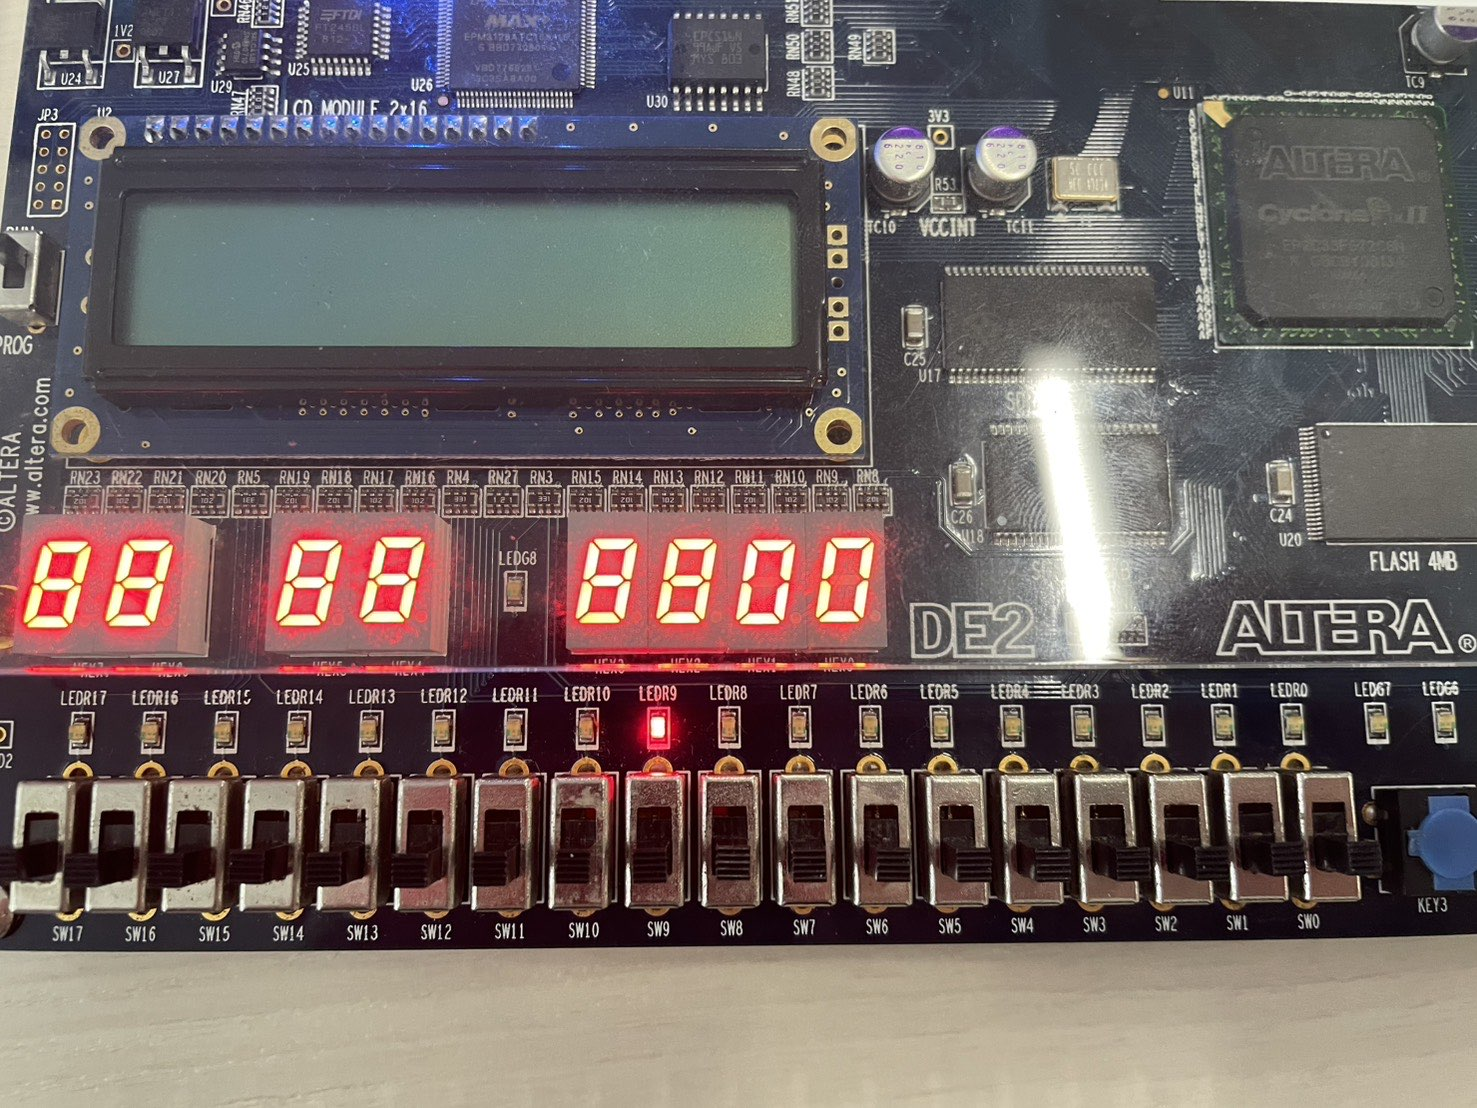
\includegraphics[width=\linewidth,height=3.5cm,keepaspectratio]{images/num-0.jpg}\caption*{\texttt{0}}\end{subfigure}\hfill
  \begin{subfigure}[b]{0.22\linewidth}\centering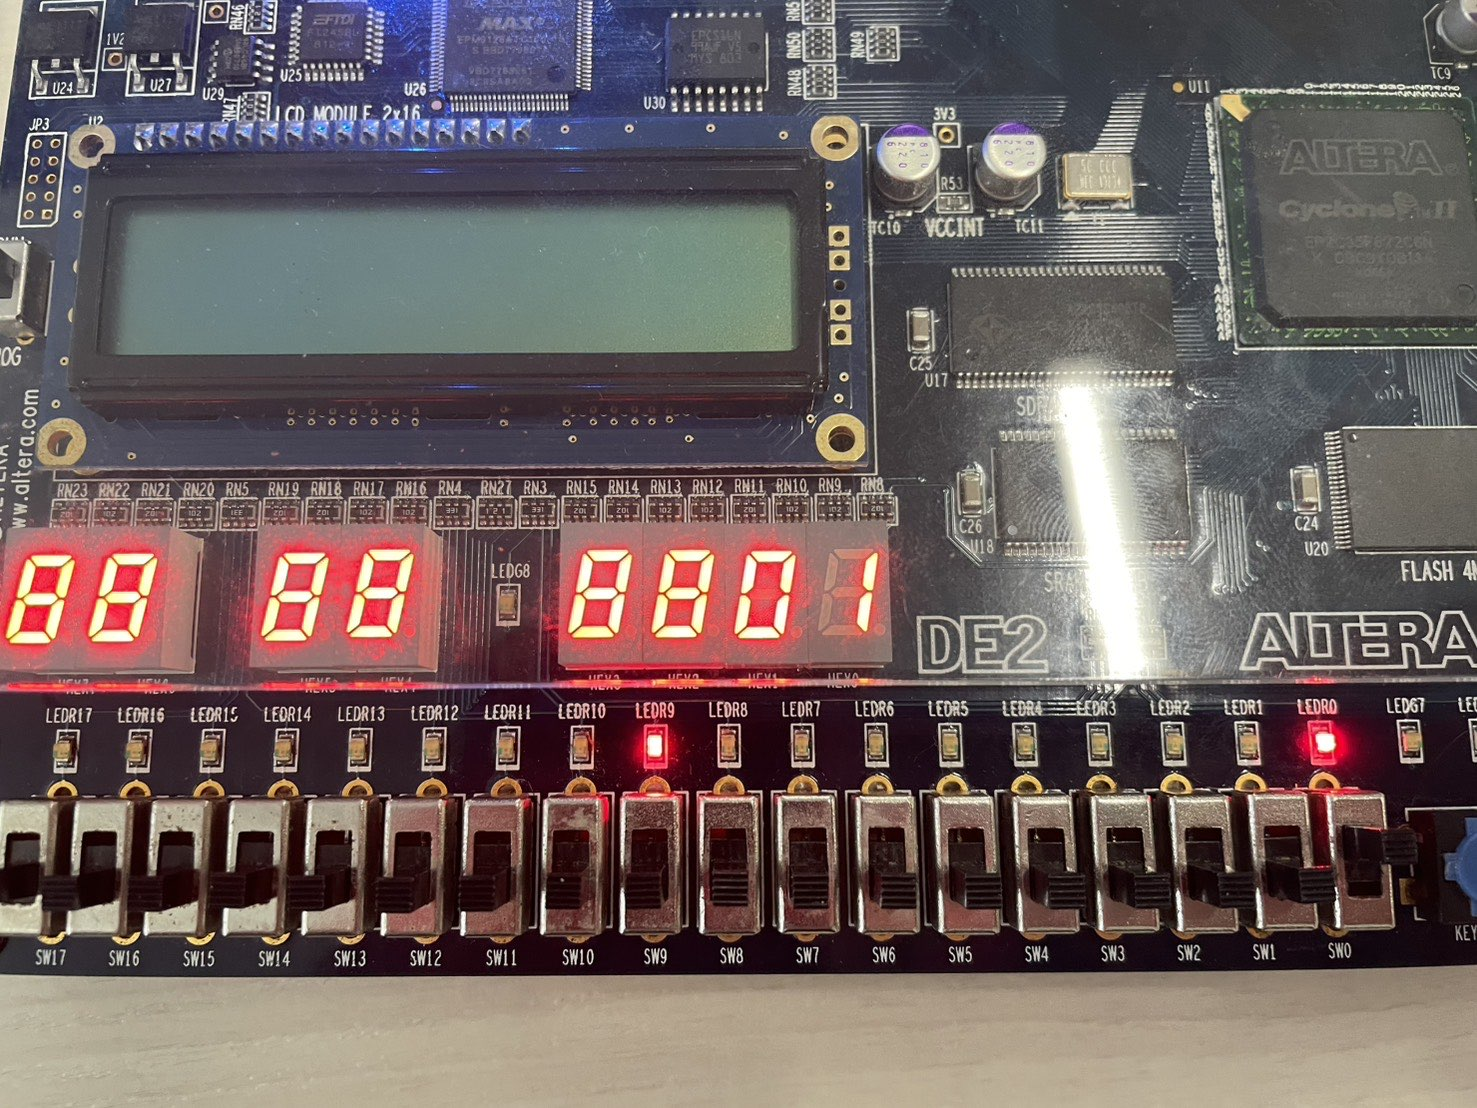
\includegraphics[width=\linewidth,height=3.5cm,keepaspectratio]{images/num-1.jpg}\caption*{\texttt{1}}\end{subfigure}\hfill
  \begin{subfigure}[b]{0.22\linewidth}\centering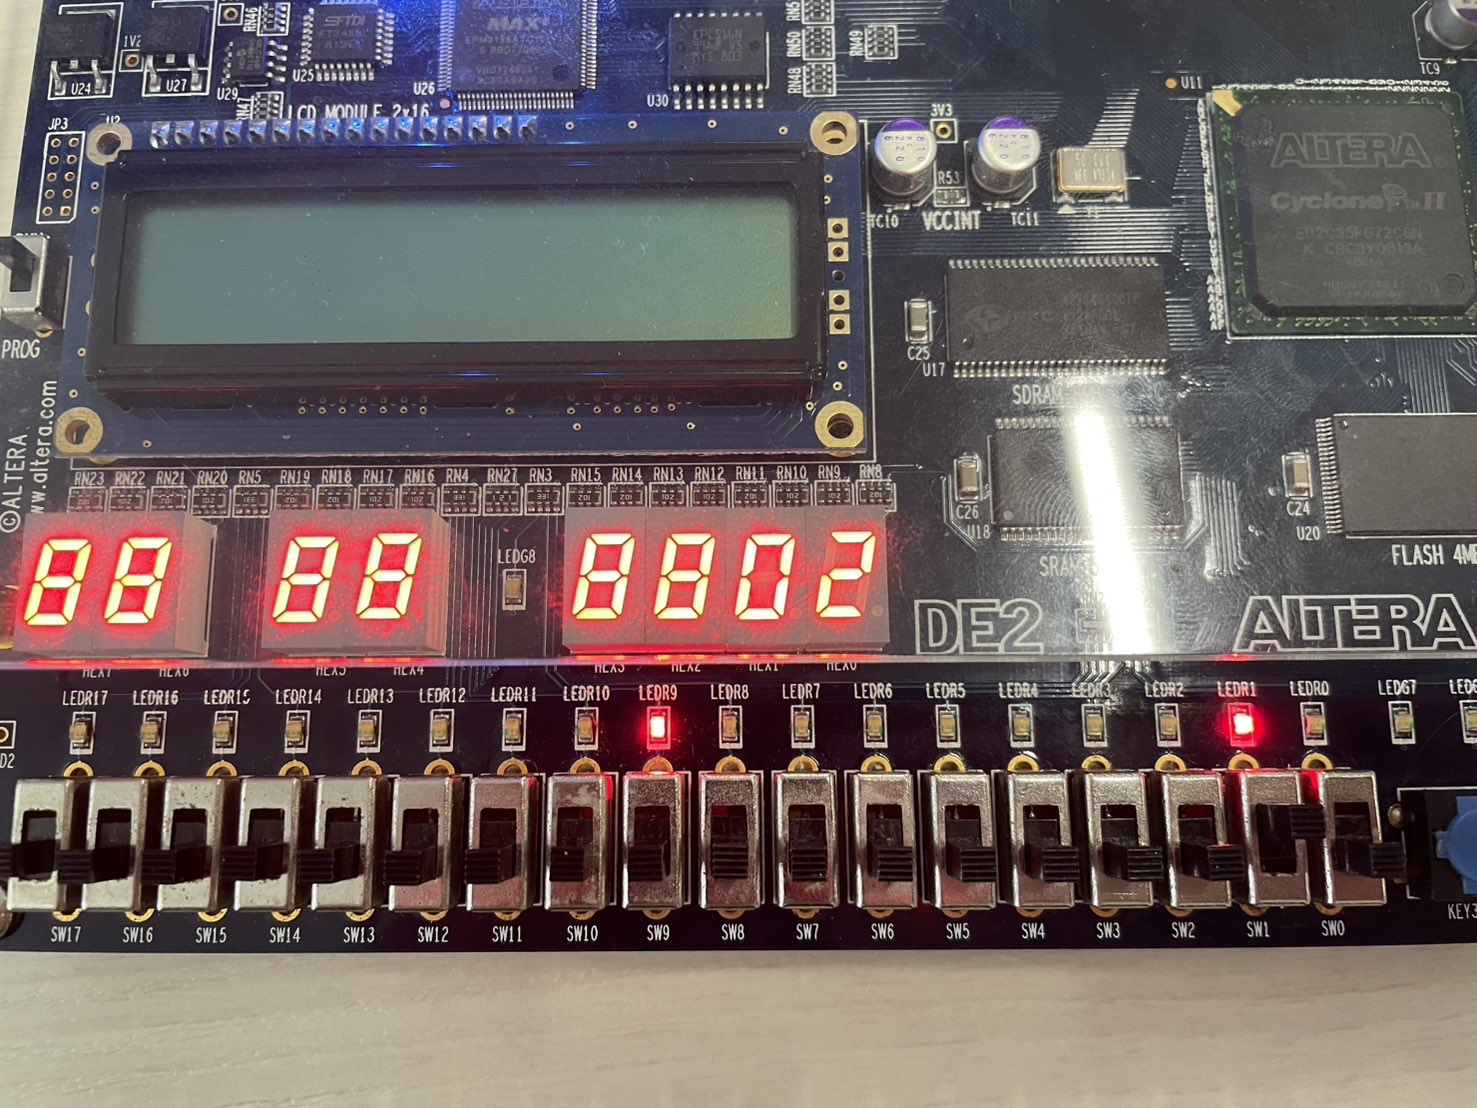
\includegraphics[width=\linewidth,height=3.5cm,keepaspectratio]{images/num-2.jpg}\caption*{\texttt{2}}\end{subfigure}\hfill
  \begin{subfigure}[b]{0.22\linewidth}\centering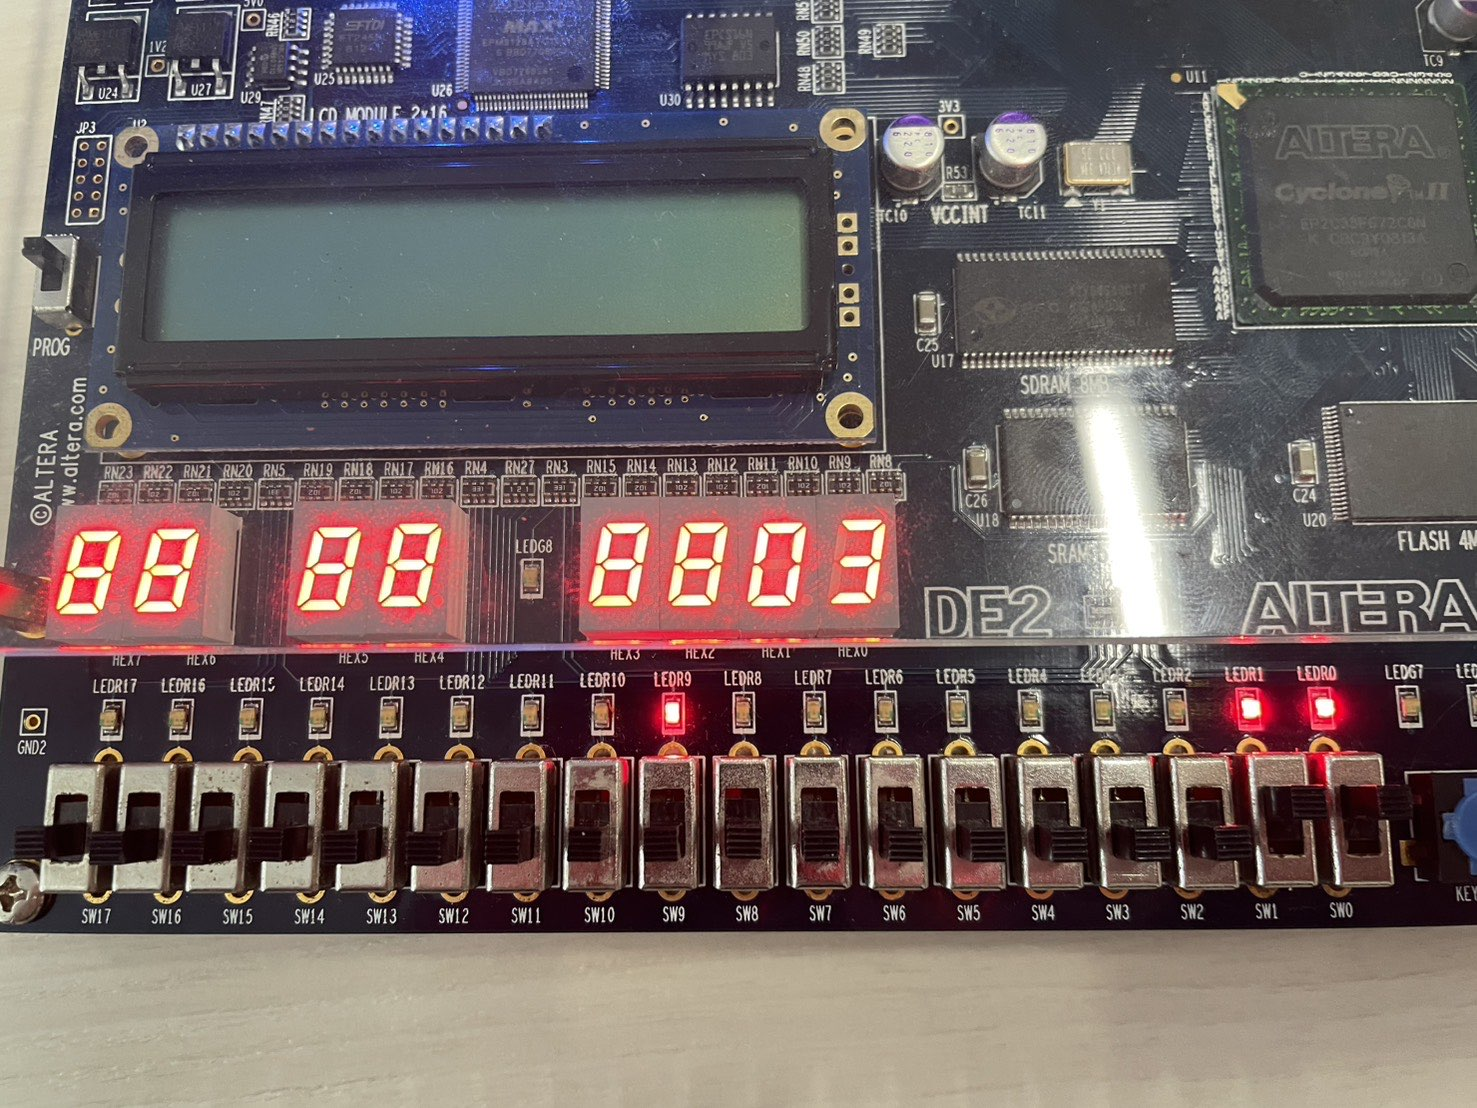
\includegraphics[width=\linewidth,height=3.5cm,keepaspectratio]{images/num-3.jpg}\caption*{\texttt{3}}\end{subfigure}\\[2ex]
  \begin{subfigure}[b]{0.22\linewidth}\centering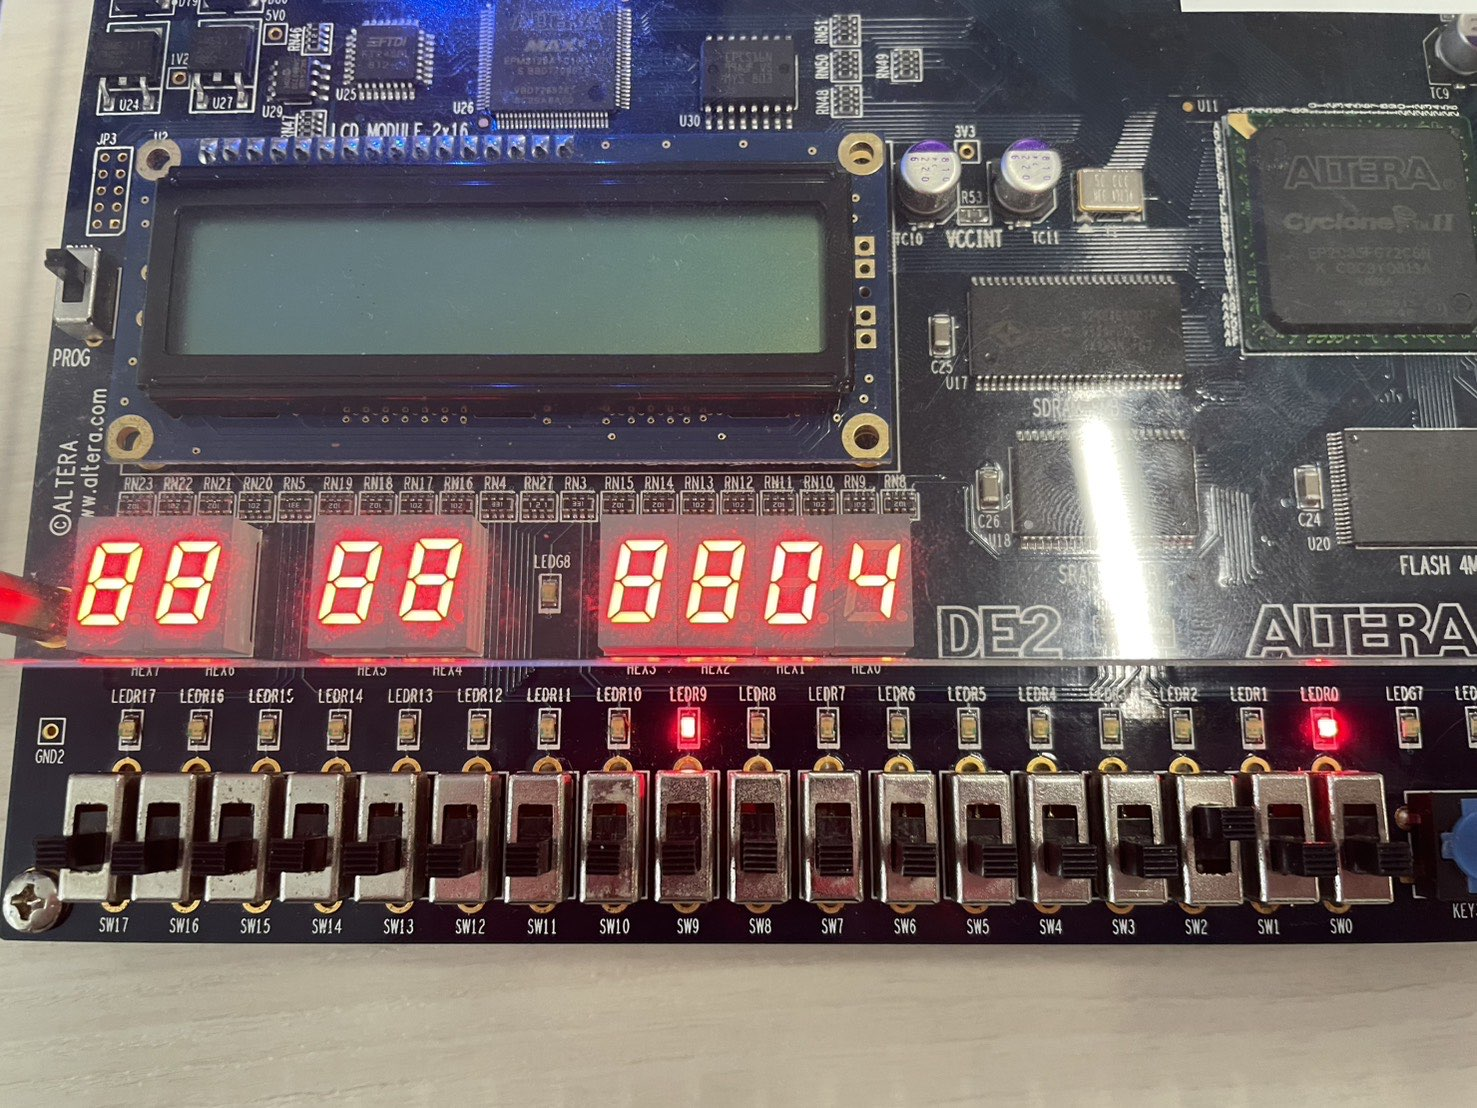
\includegraphics[width=\linewidth,height=3.5cm,keepaspectratio]{images/num-4.jpg}\caption*{\texttt{4}}\end{subfigure}\hfill
  \begin{subfigure}[b]{0.22\linewidth}\centering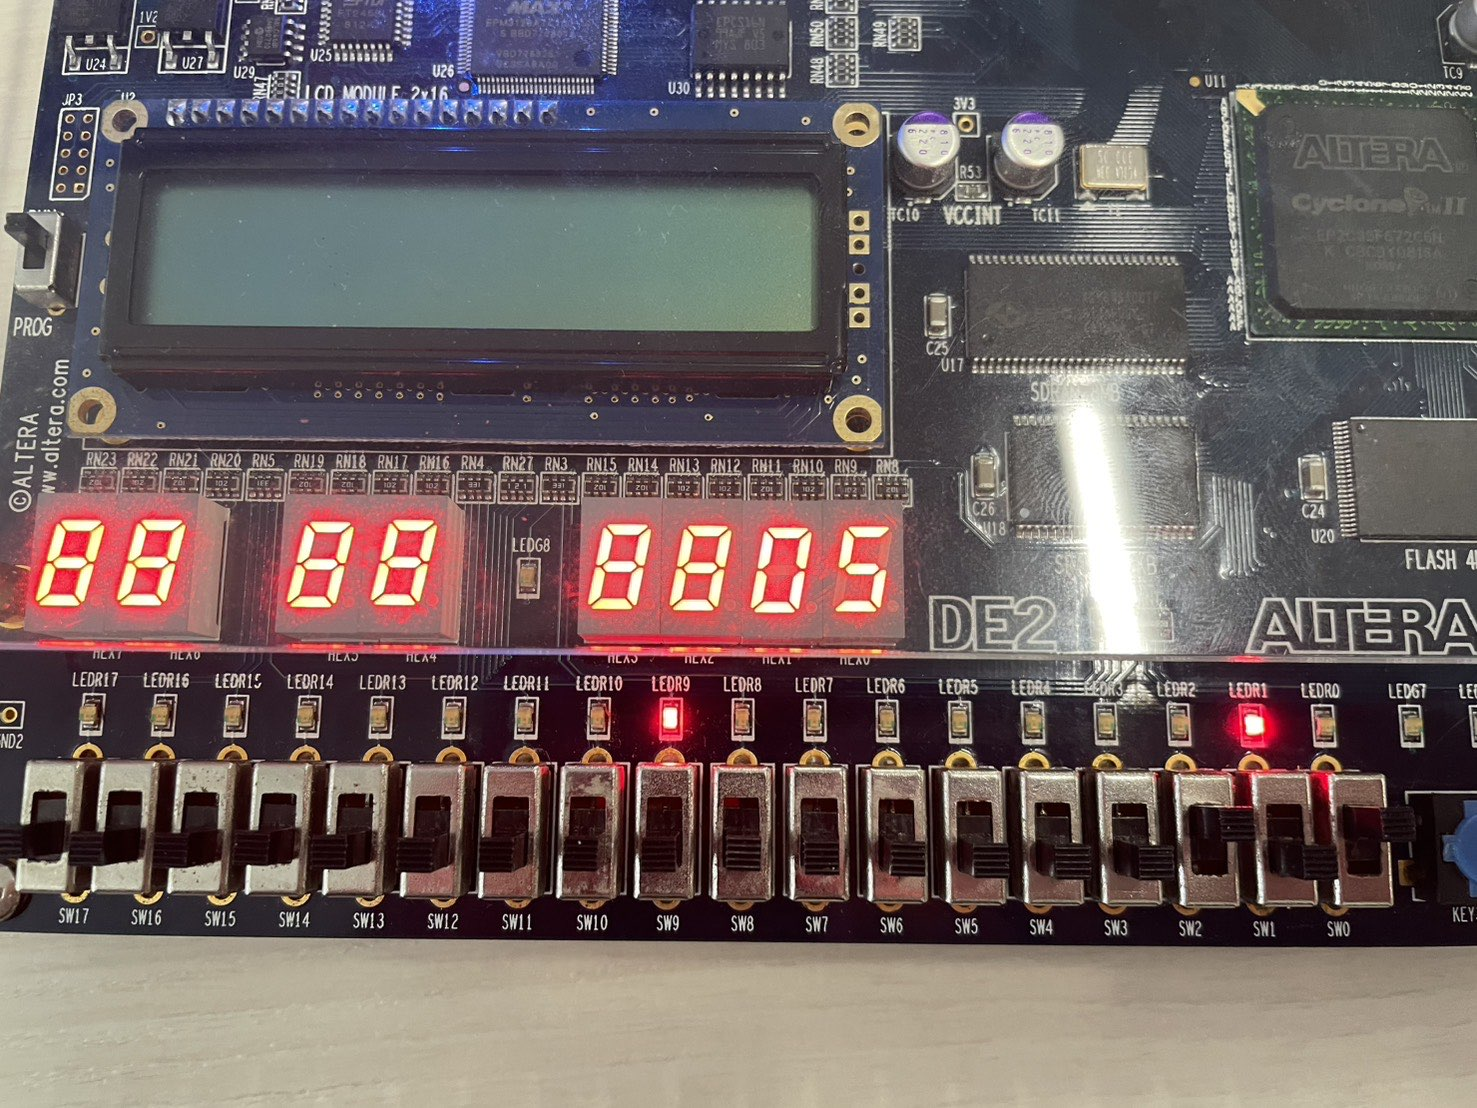
\includegraphics[width=\linewidth,height=3.5cm,keepaspectratio]{images/num-5.jpg}\caption*{\texttt{5}}\end{subfigure}\hfill
  \begin{subfigure}[b]{0.22\linewidth}\centering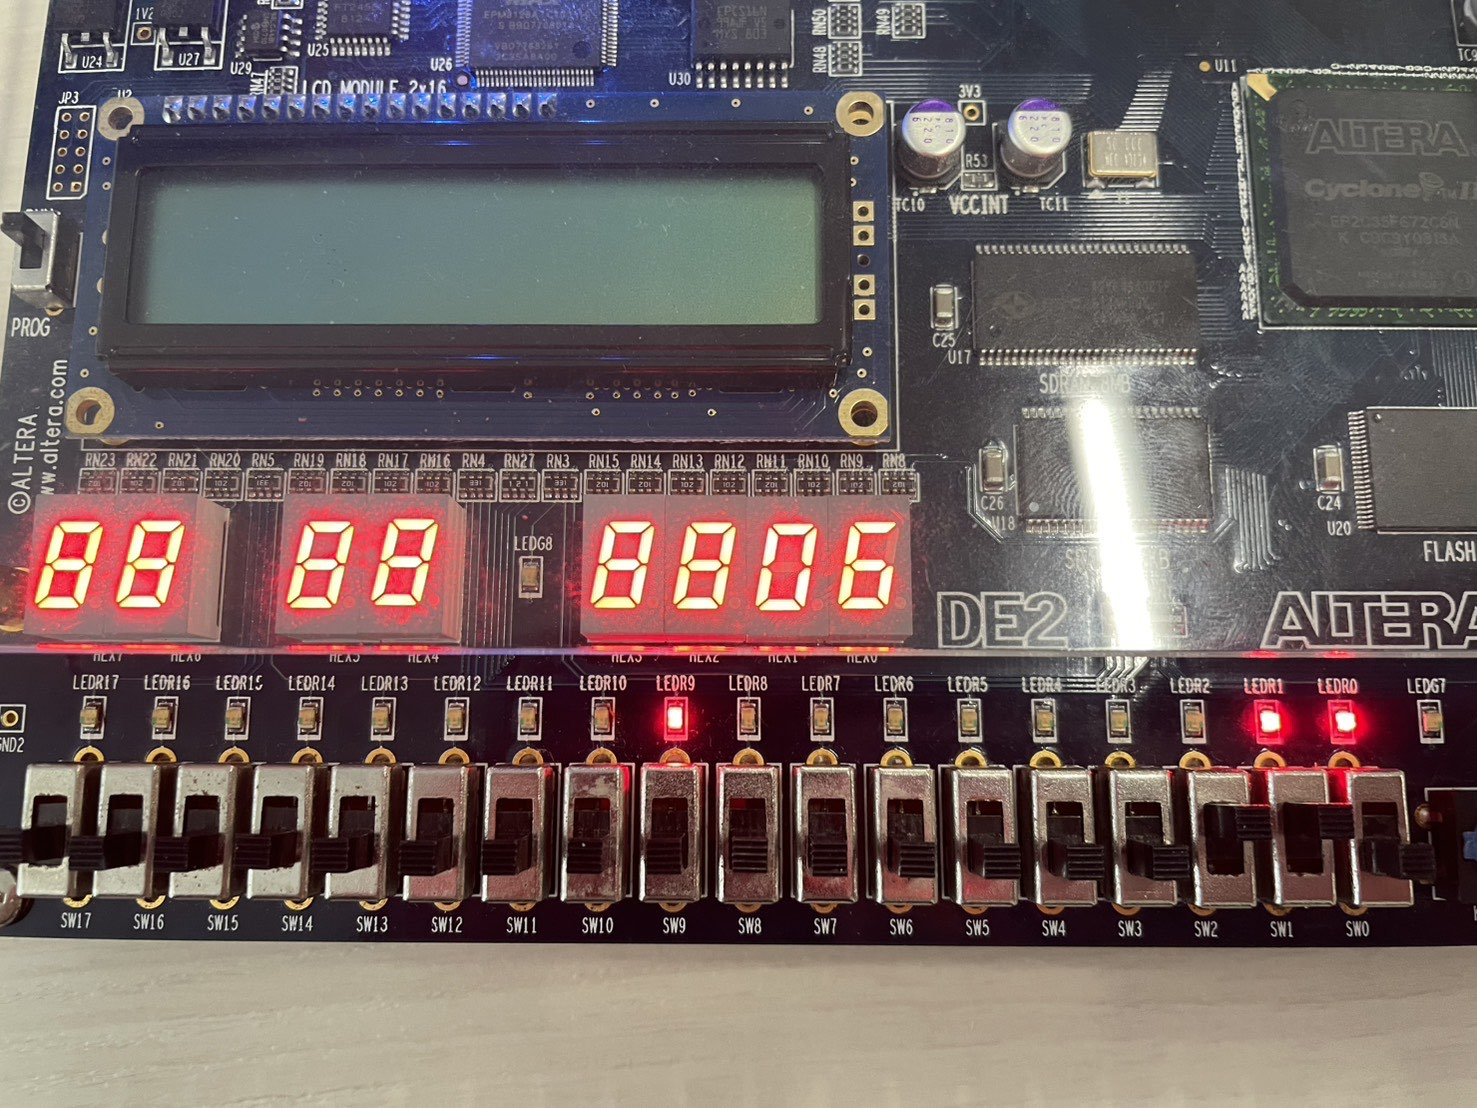
\includegraphics[width=\linewidth,height=3.5cm,keepaspectratio]{images/num-6.jpg}\caption*{\texttt{6}}\end{subfigure}\hfill
  \begin{subfigure}[b]{0.22\linewidth}\centering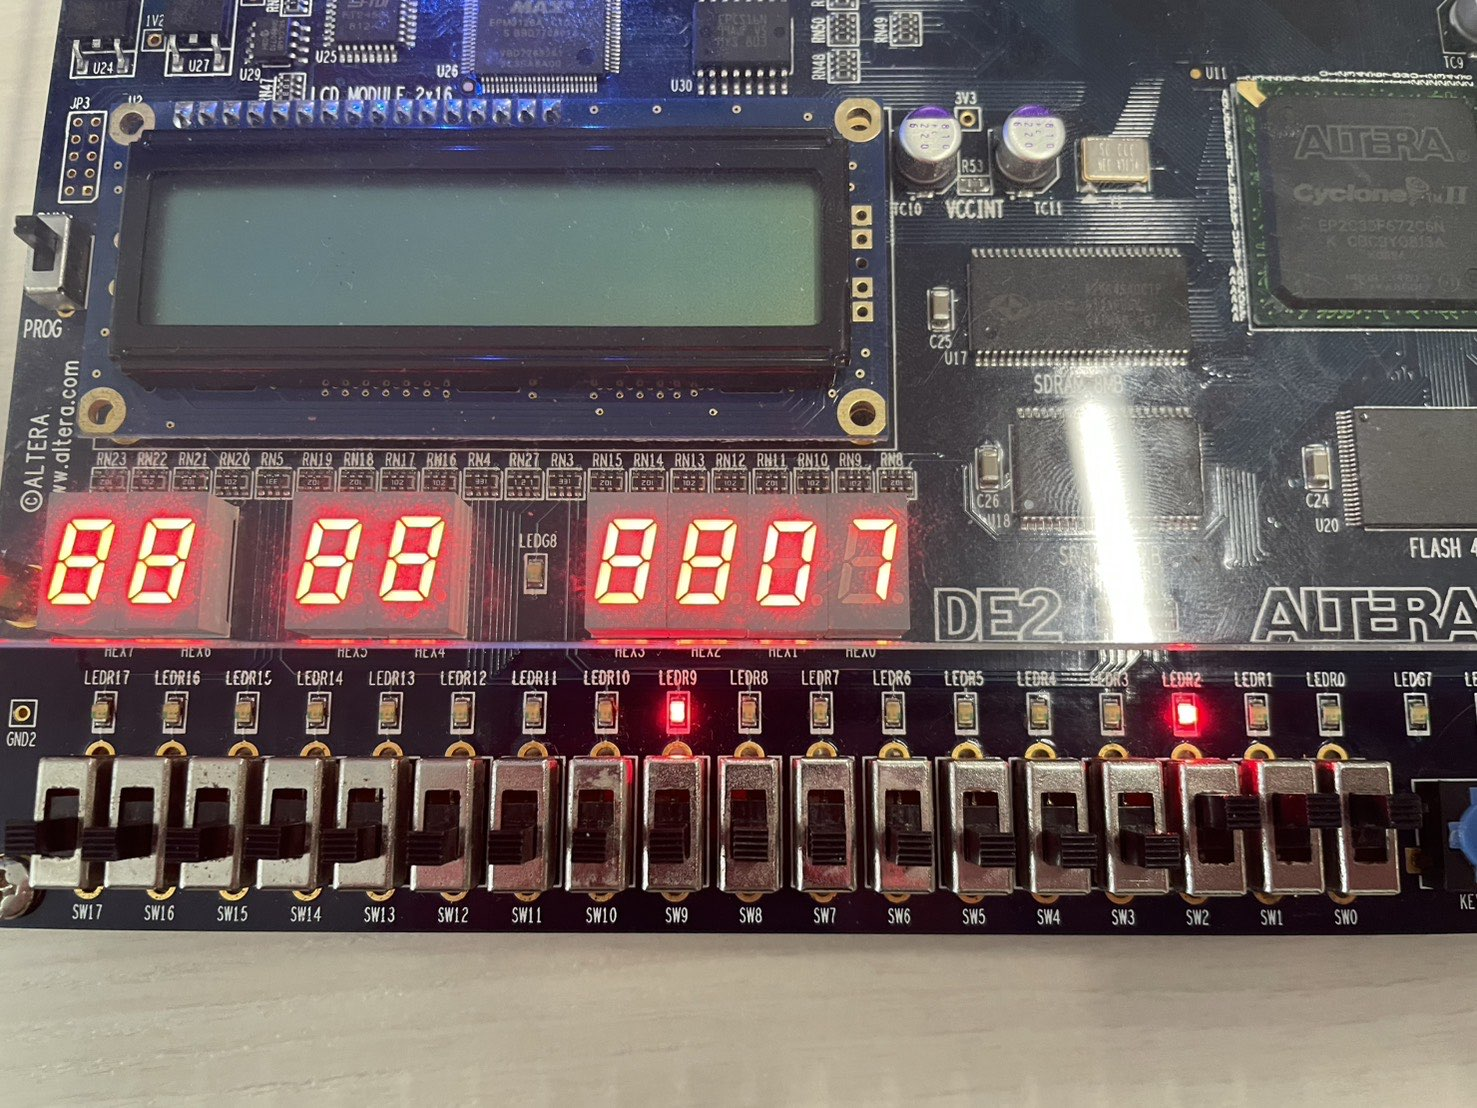
\includegraphics[width=\linewidth,height=3.5cm,keepaspectratio]{images/num-7.jpg}\caption*{\texttt{7}}\end{subfigure}\\[2ex]
  \begin{subfigure}[b]{0.22\linewidth}\centering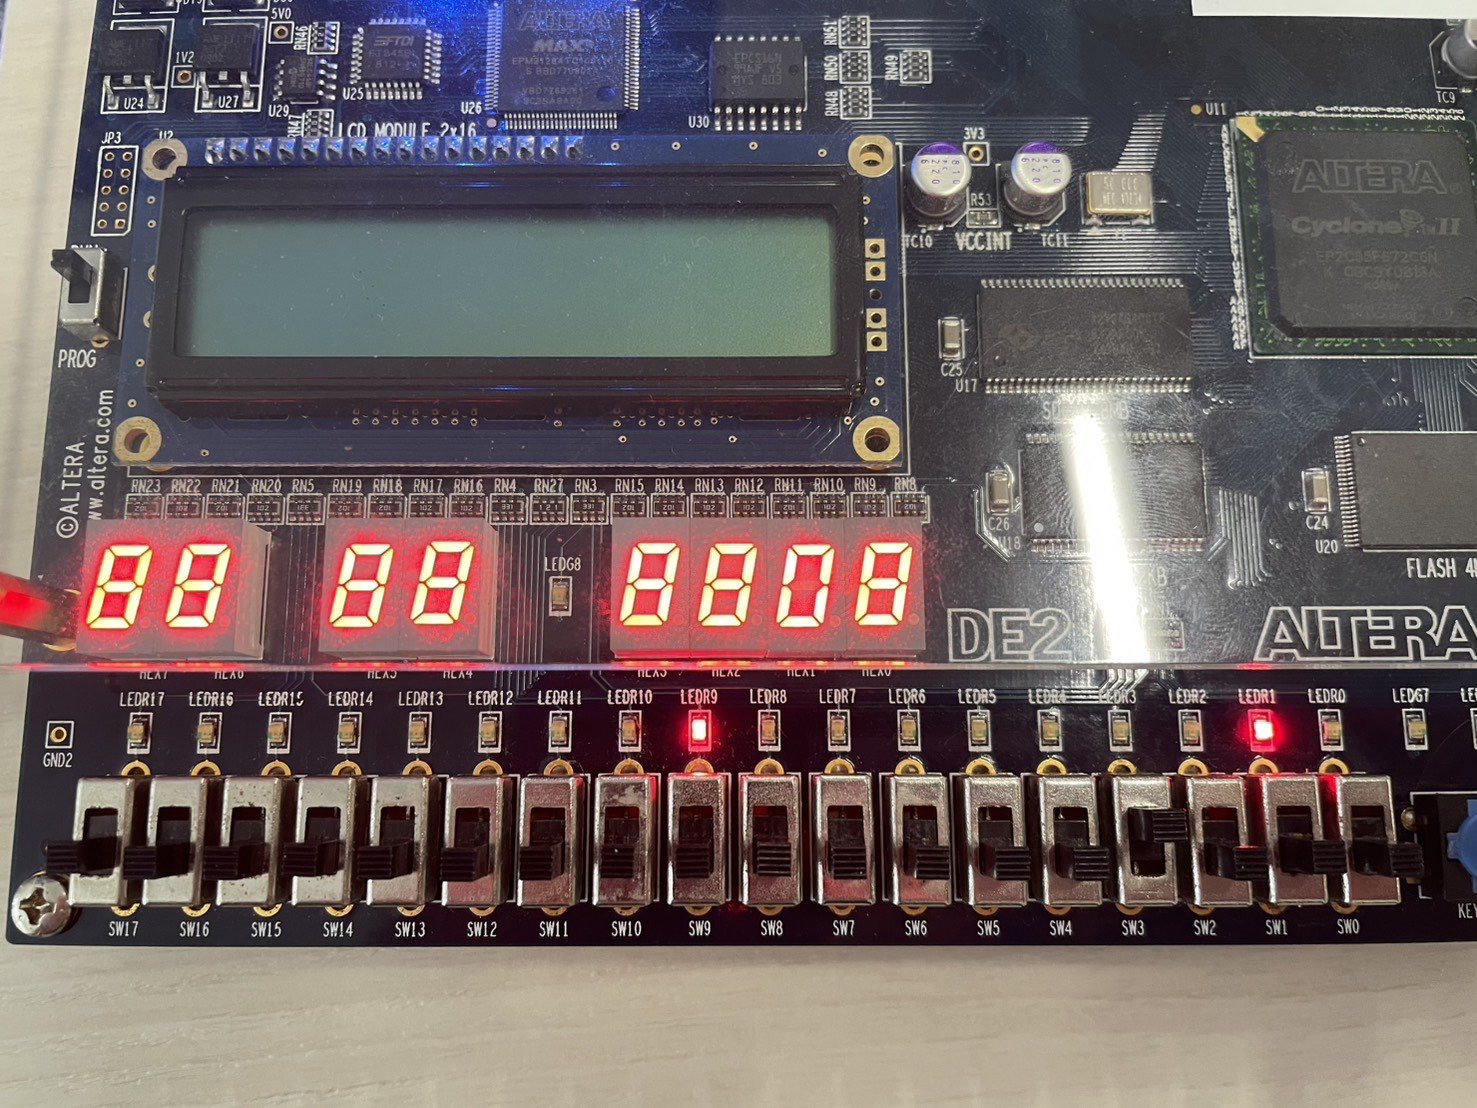
\includegraphics[width=\linewidth,height=3.5cm,keepaspectratio]{images/num-8.jpg}\caption*{\texttt{8}}\end{subfigure}\hfill
  \begin{subfigure}[b]{0.22\linewidth}\centering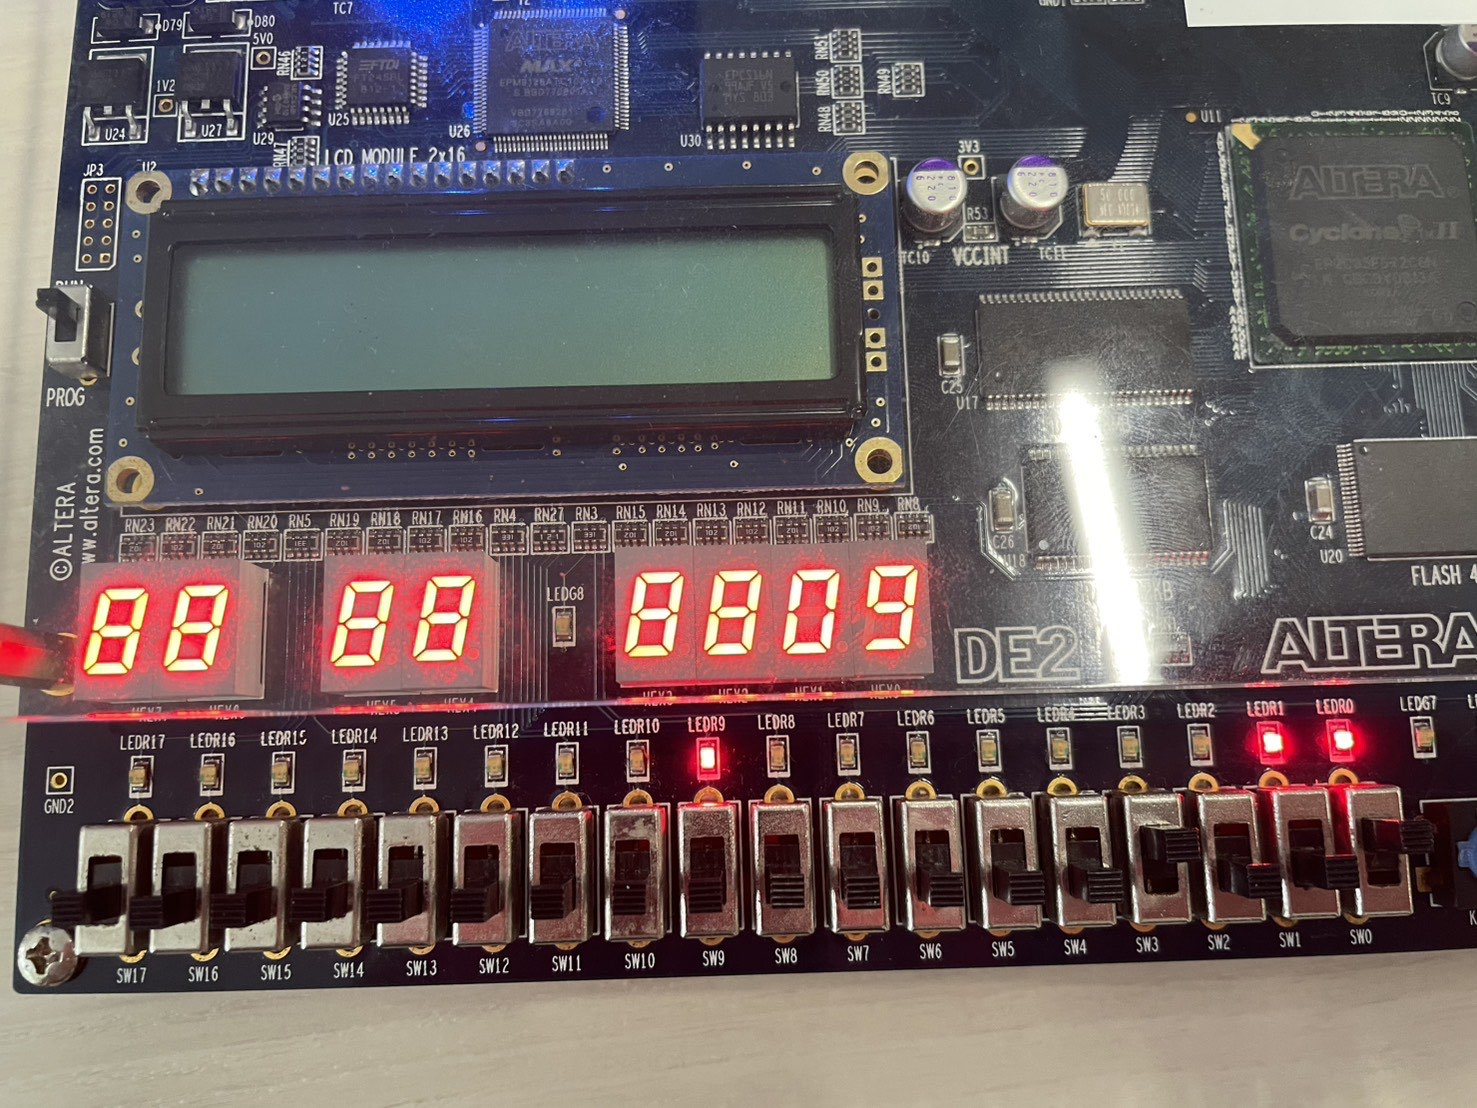
\includegraphics[width=\linewidth,height=3.5cm,keepaspectratio]{images/num-9.jpg}\caption*{\texttt{9}}\end{subfigure}\hfill
  \begin{subfigure}[b]{0.22\linewidth}\centering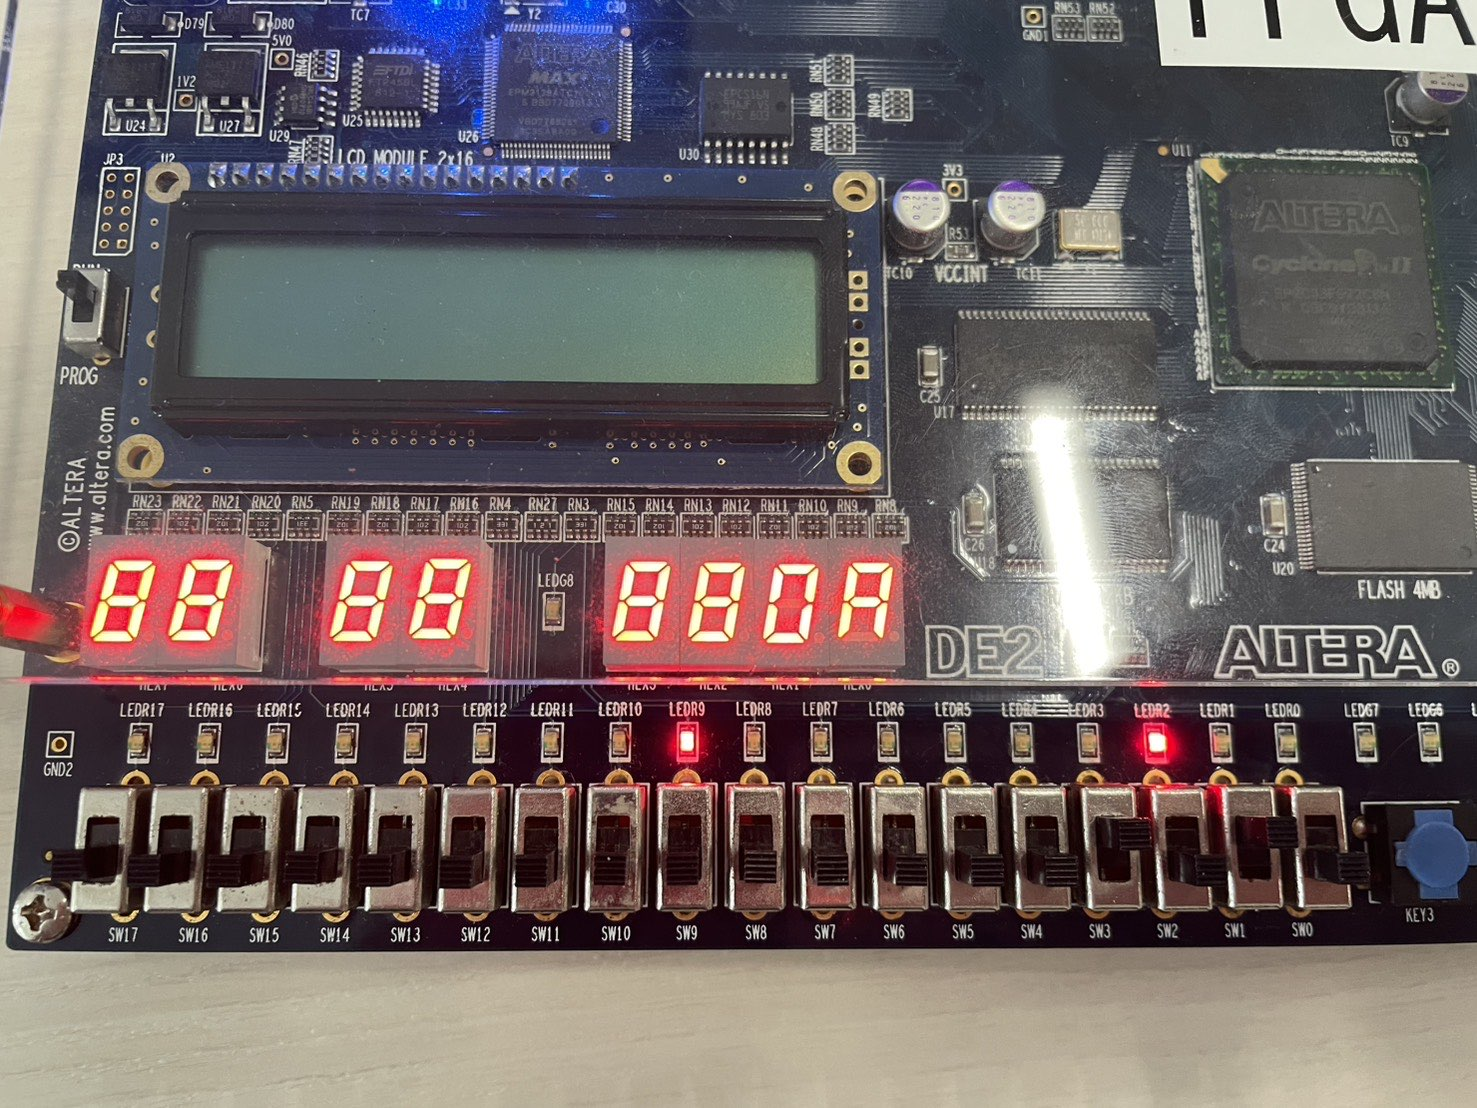
\includegraphics[width=\linewidth,height=3.5cm,keepaspectratio]{images/num-a.jpg}\caption*{\texttt{A}}\end{subfigure}\hfill
  \begin{subfigure}[b]{0.22\linewidth}\centering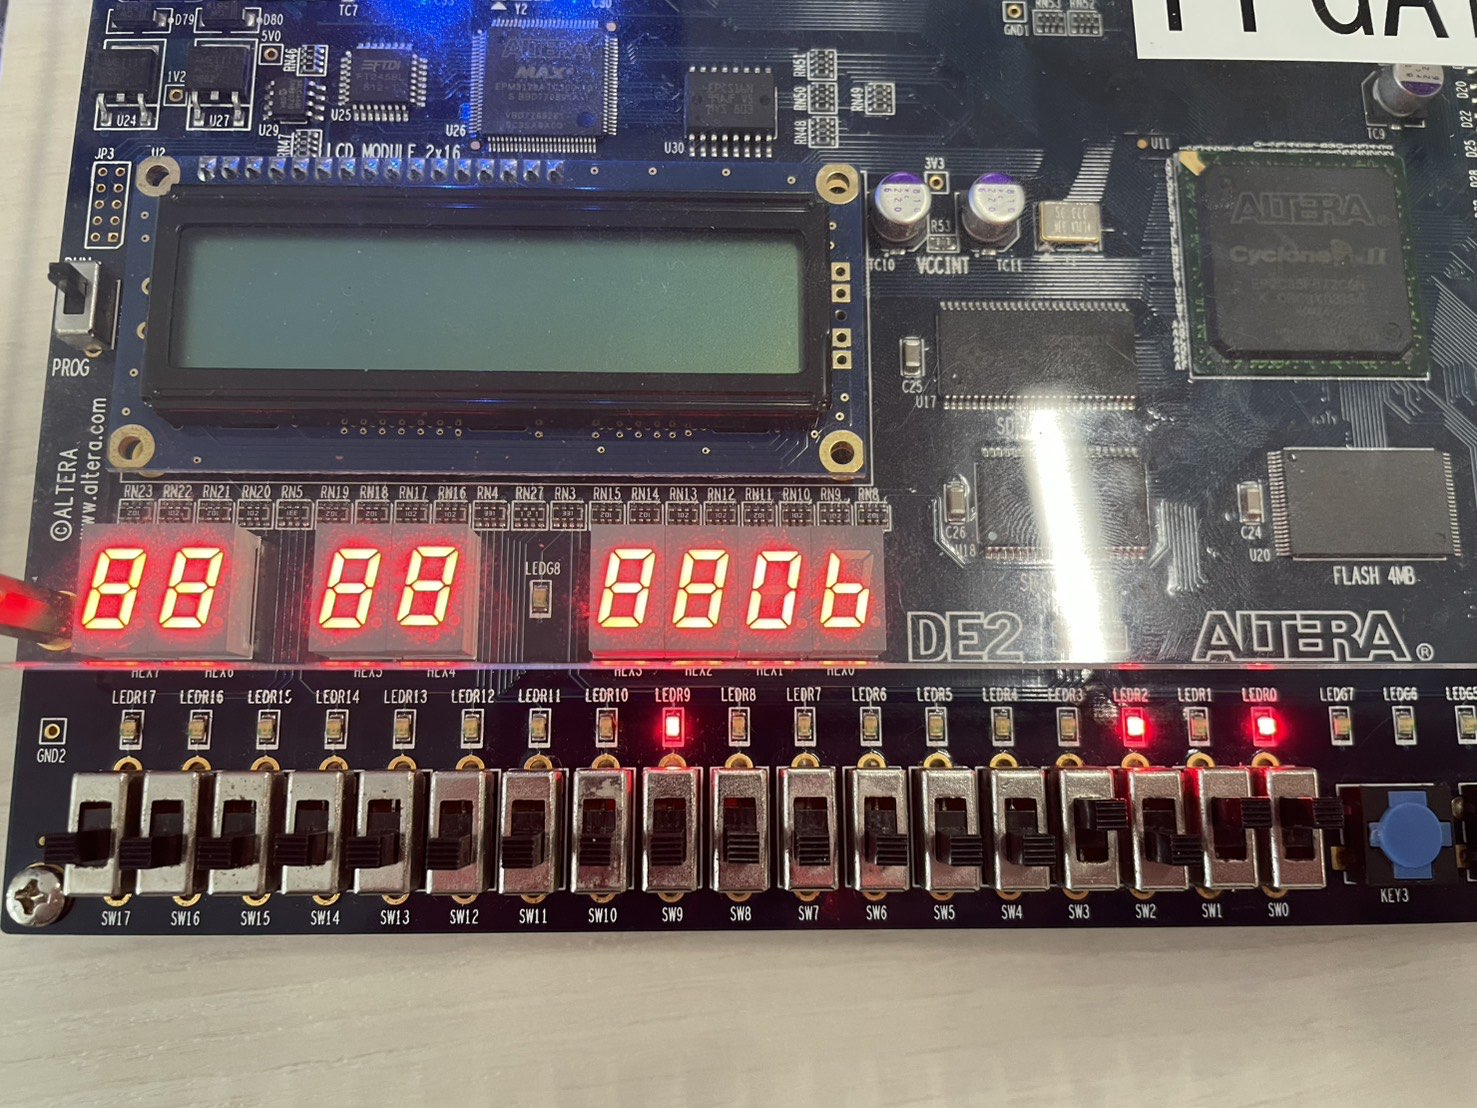
\includegraphics[width=\linewidth,height=3.5cm,keepaspectratio]{images/num-b.jpg}\caption*{\texttt{b}}\end{subfigure}\\[2ex]
  \begin{subfigure}[b]{0.22\linewidth}\centering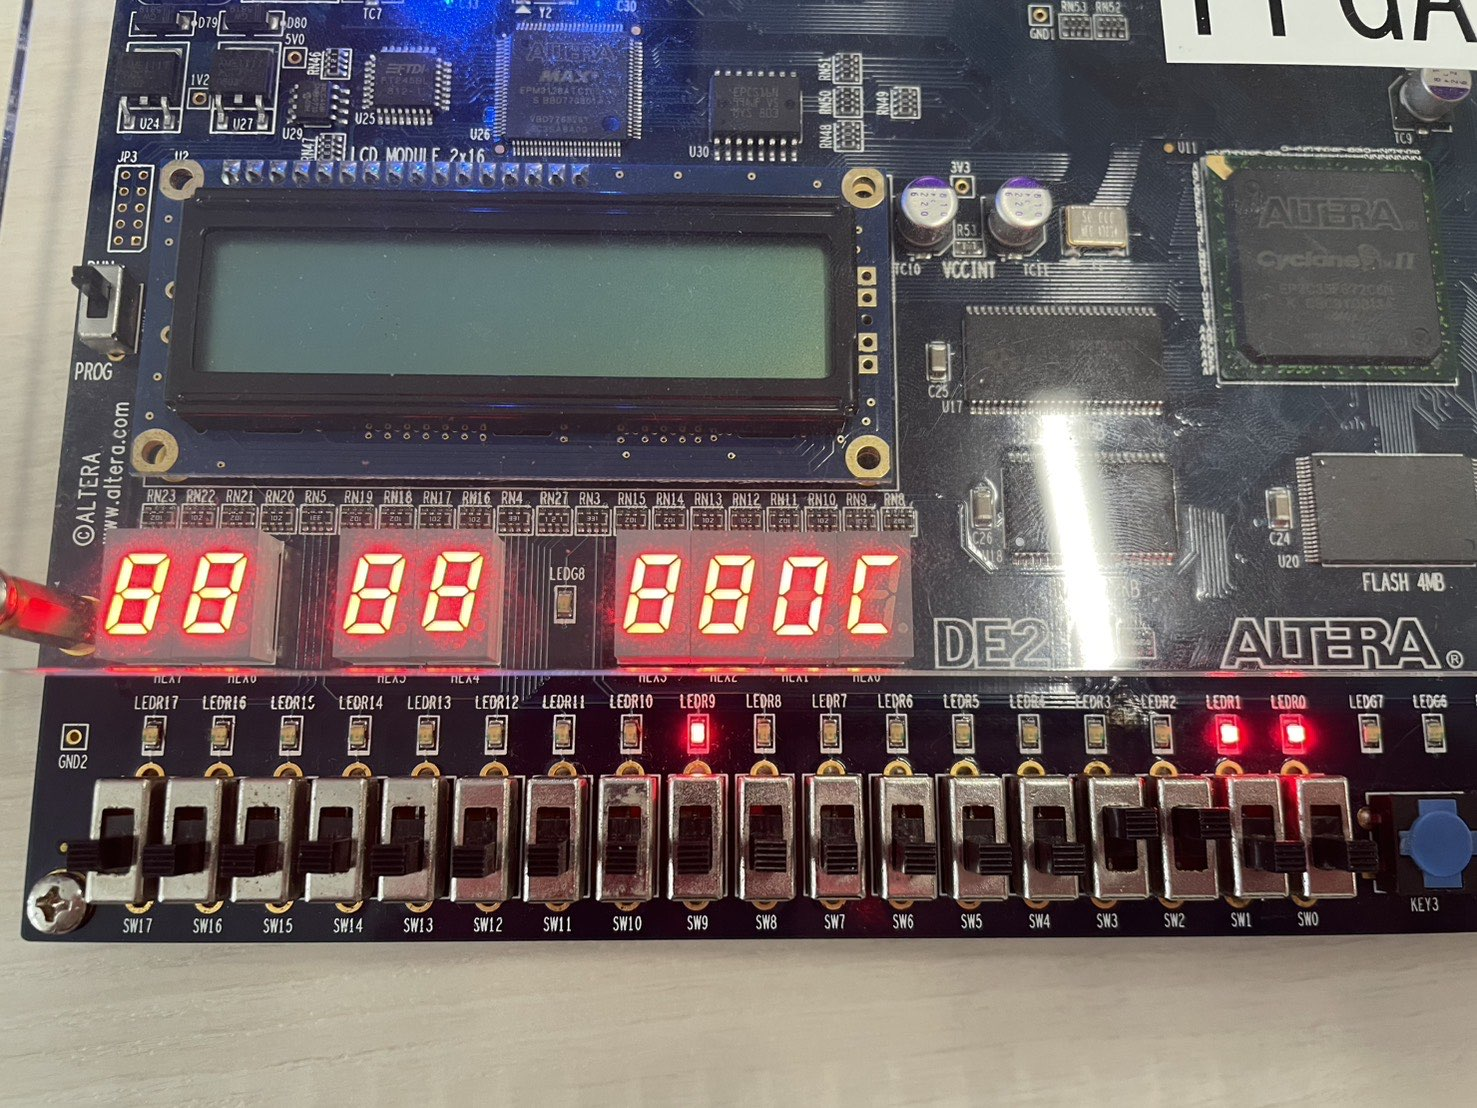
\includegraphics[width=\linewidth,height=3.5cm,keepaspectratio]{images/num-c.jpg}\caption*{\texttt{C}}\end{subfigure}\hfill
  \begin{subfigure}[b]{0.22\linewidth}\centering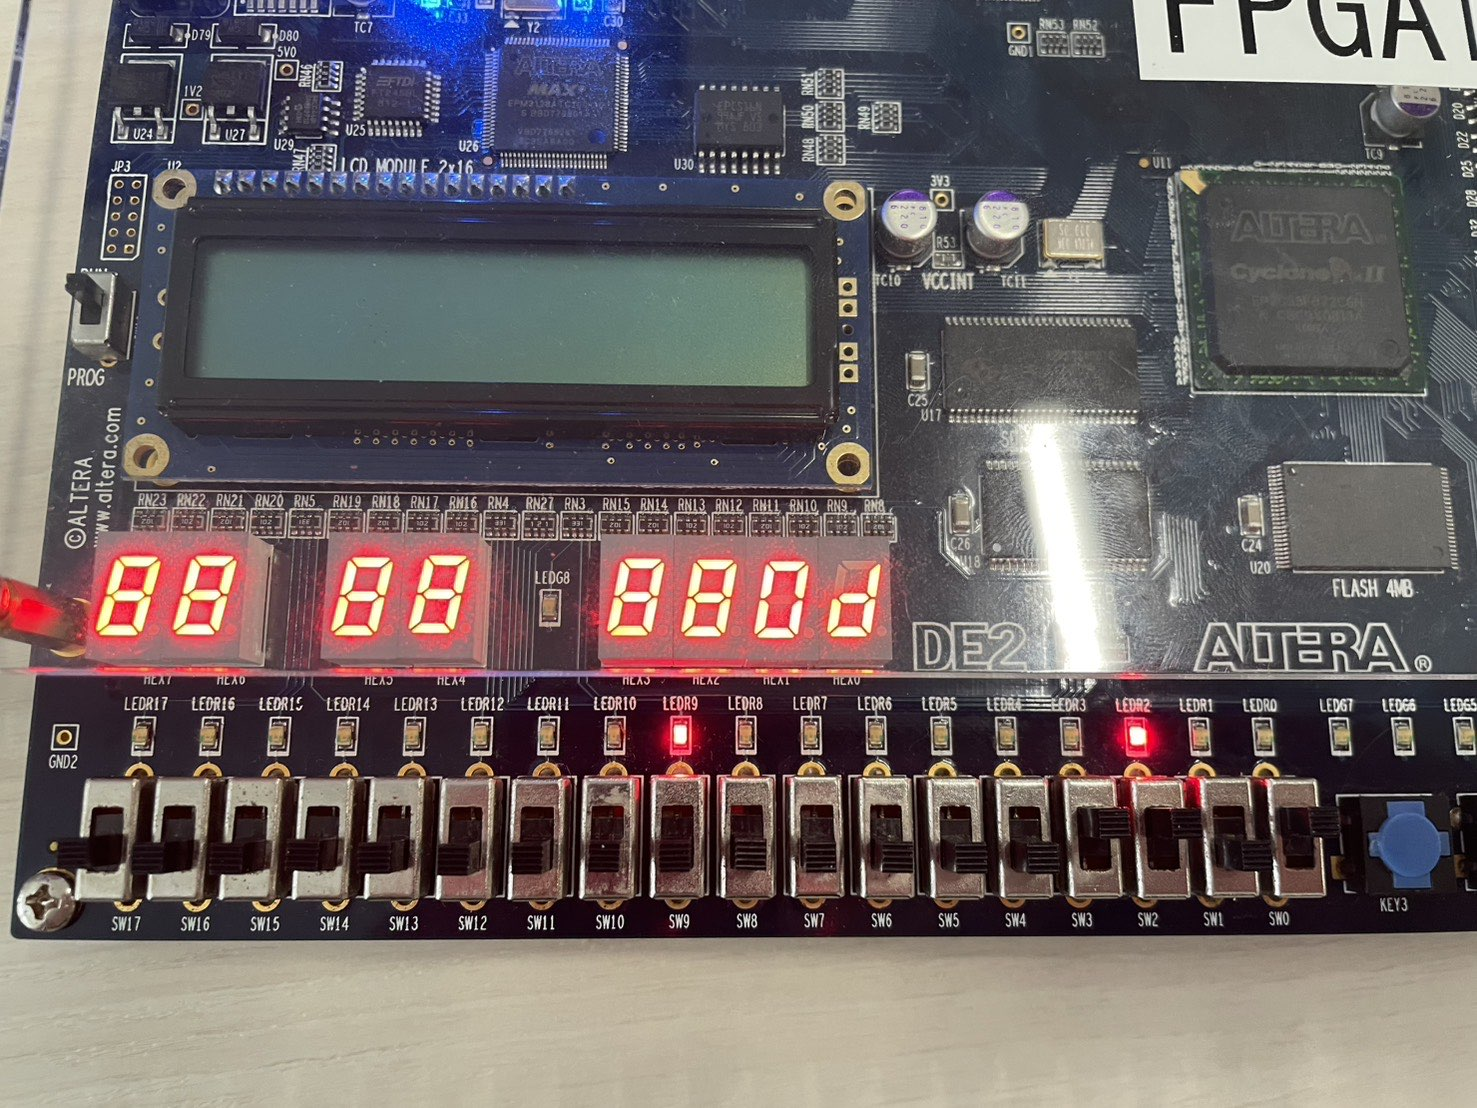
\includegraphics[width=\linewidth,height=3.5cm,keepaspectratio]{images/num-d.jpg}\caption*{\texttt{d}}\end{subfigure}\hfill
  \begin{subfigure}[b]{0.22\linewidth}\centering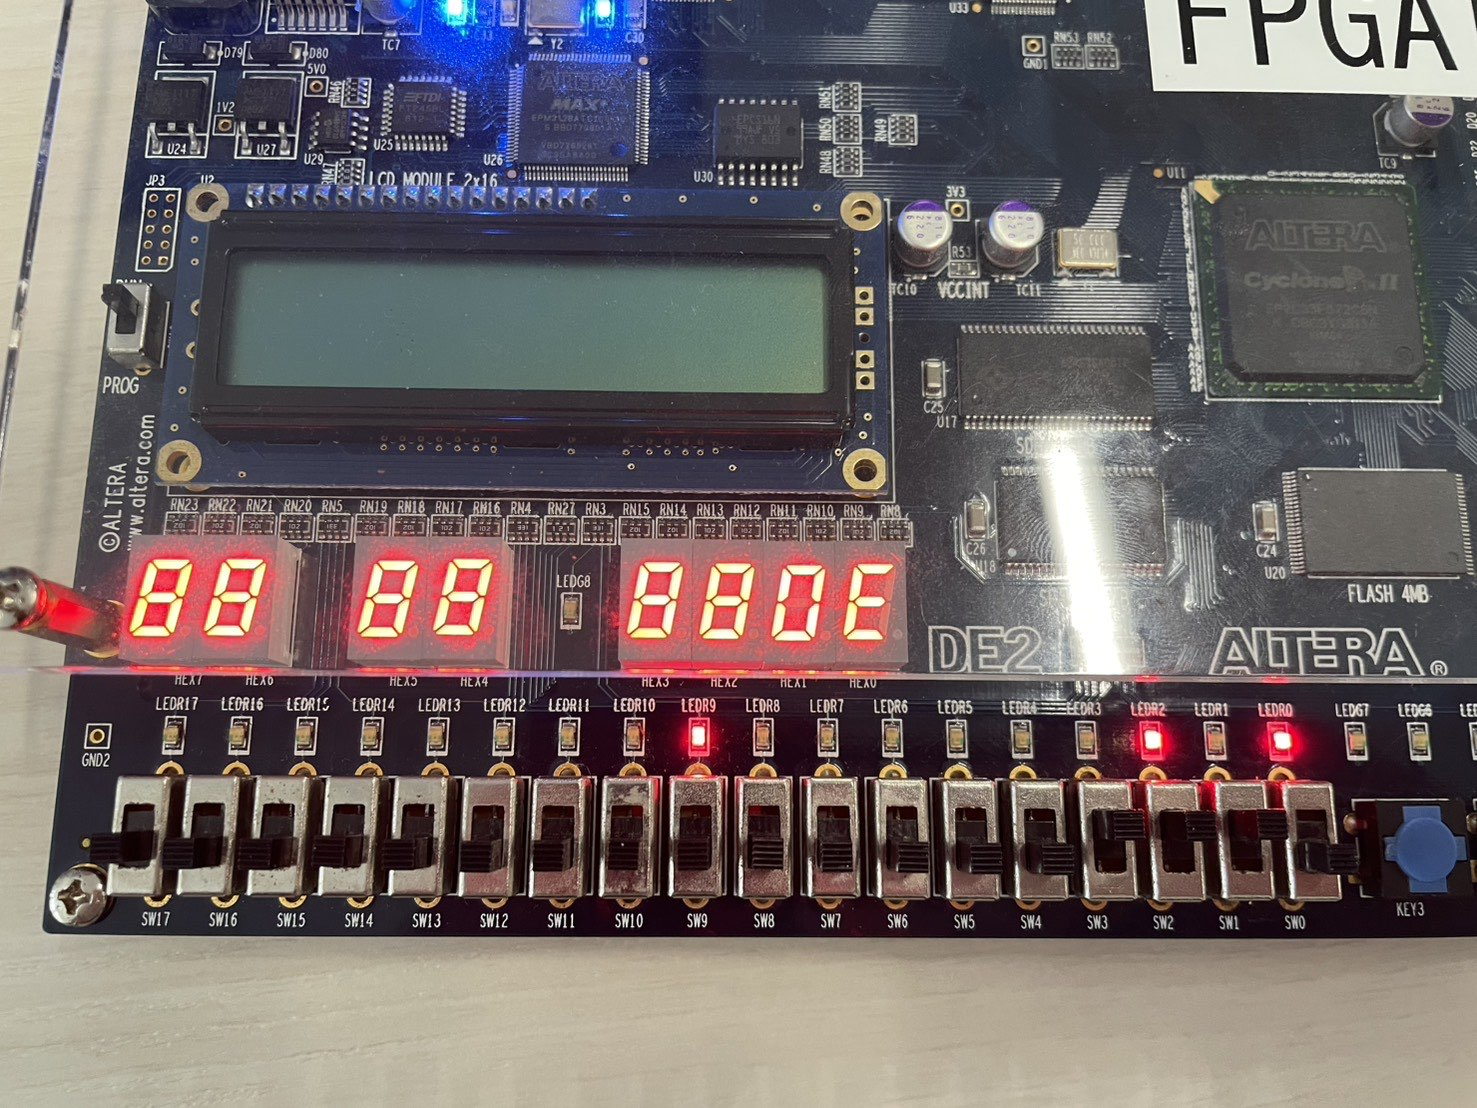
\includegraphics[width=\linewidth,height=3.5cm,keepaspectratio]{images/num-e.jpg}\caption*{\texttt{E}}\end{subfigure}\hfill
  \begin{subfigure}[b]{0.22\linewidth}\centering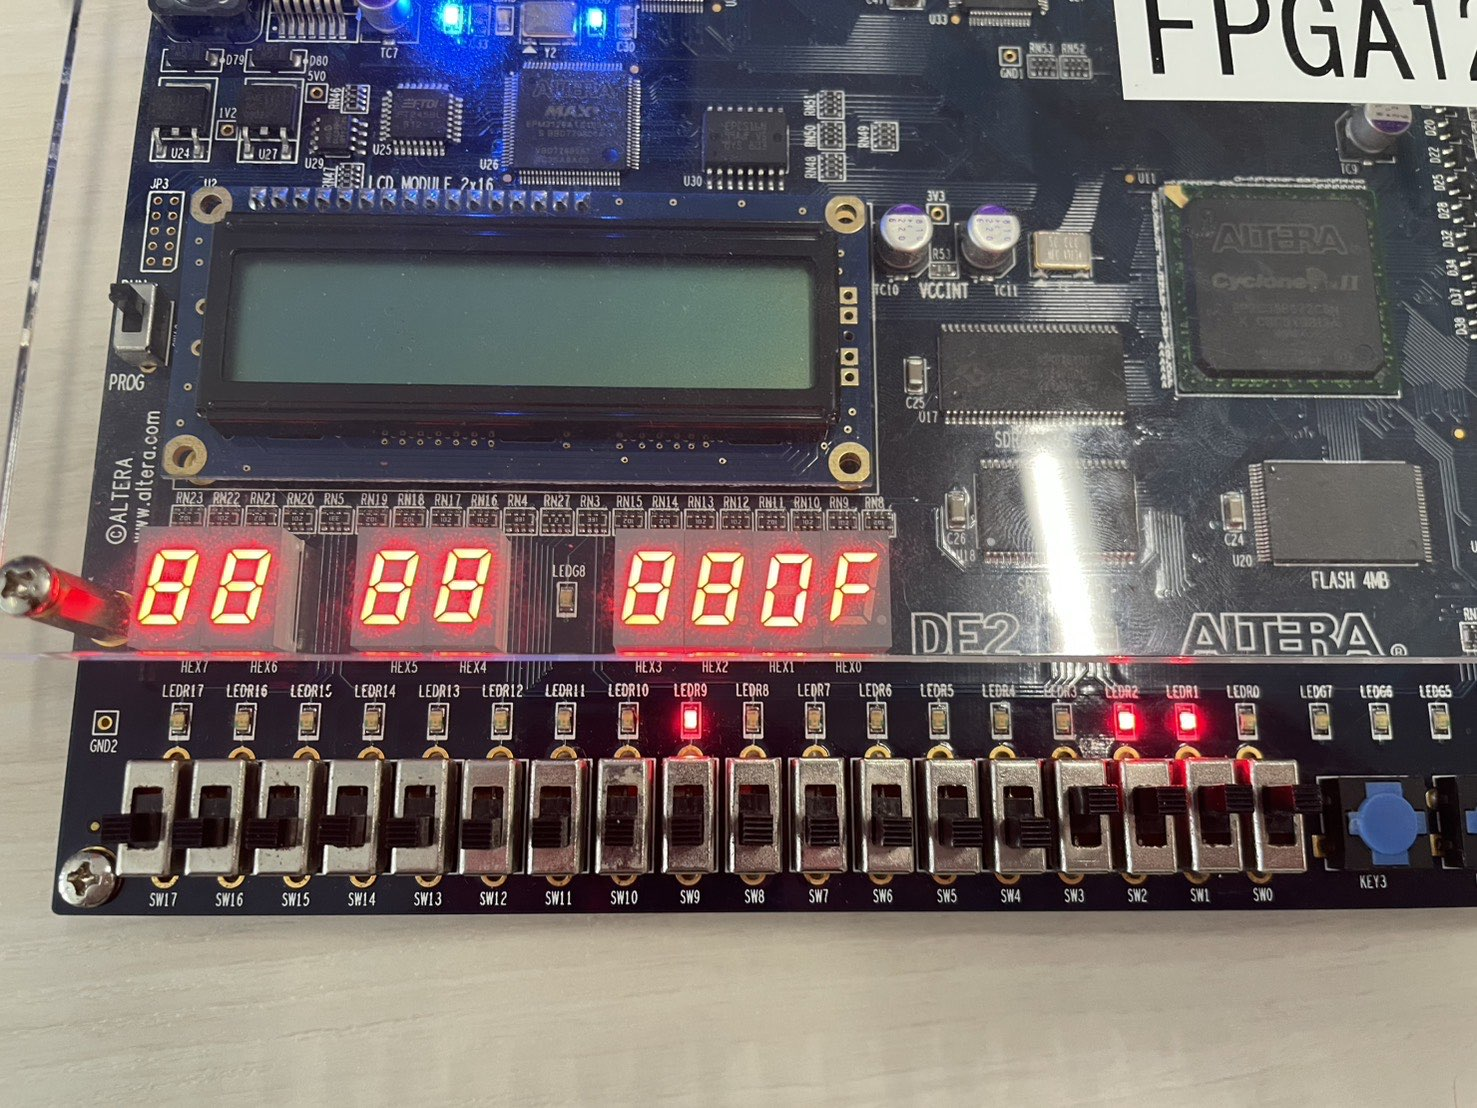
\includegraphics[width=\linewidth,height=3.5cm,keepaspectratio]{images/num-f.jpg}\caption*{\texttt{F}}\end{subfigure}
  \caption{課題２：7セグメント表示結果（0〜F）}\label{fig:hex2seg7-result}
\end{figure}

\newpage
\subsection{課題３}

課題３では \texttt{hex2seg7} コンポーネントを２つ使用し、
\texttt{SW[7:4]}（上位ニブル）を \texttt{HEX1} に、
\texttt{SW[3:0]}（下位ニブル）を \texttt{HEX0} に出力した。
表\ref{tab:hex2seg7-2digit}に代表的な入力に対する出力例を示す。

\begin{table}[h]
  \centering
  \caption{8ビット入力の2桁16進表示（代表例）}
  \label{tab:hex2seg7-2digit}
  \begin{tabular}{cc|cc}
    \toprule
    SW{[7:0]}（2進数） & SW（16進数） & HEX1（上位桁） & HEX0（下位桁） \\
    \midrule
    0000 0000 & \texttt{00} & \texttt{0} & \texttt{0} \\
    0000 1111 & \texttt{0F} & \texttt{0} & \texttt{F} \\
    0001 0000 & \texttt{10} & \texttt{1} & \texttt{0} \\
    0011 1010 & \texttt{3A} & \texttt{3} & \texttt{A} \\
    0101 0101 & \texttt{55} & \texttt{5} & \texttt{5} \\
    1000 0000 & \texttt{80} & \texttt{8} & \texttt{0} \\
    1010 1011 & \texttt{AB} & \texttt{A} & \texttt{b} \\
    1100 1101 & \texttt{CD} & \texttt{C} & \texttt{d} \\
    1110 1111 & \texttt{EF} & \texttt{E} & \texttt{F} \\
    1111 1111 & \texttt{FF} & \texttt{F} & \texttt{F} \\
    \bottomrule
  \end{tabular}
\end{table}

図\ref{fig:hex2seg7-check}に、実際のFPGAボード上での動作確認結果を示す。

\begin{figure}[H]
  \centering
  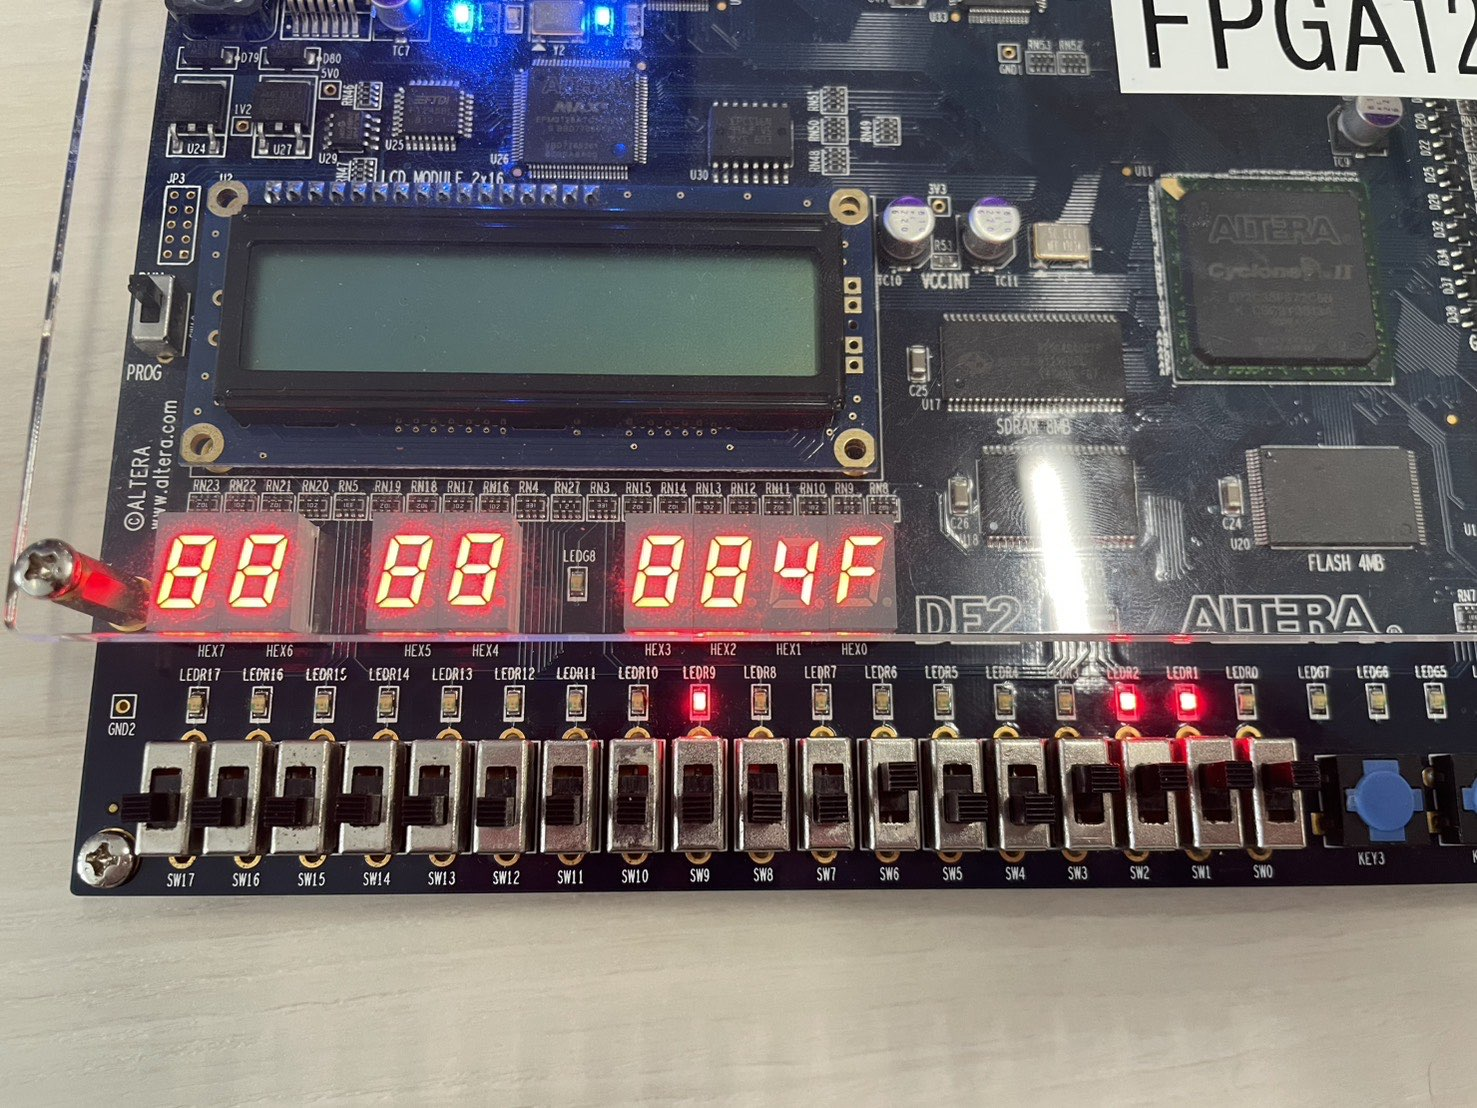
\includegraphics[width=0.5\linewidth]{images/num-check.jpg}
  \caption{課題３：2桁16進表示の動作確認}
  \label{fig:hex2seg7-check}
\end{figure}

\subsection{課題４}

表\ref{tab:compare2bits}に２ビット比較回路の真理値表を示す。
入力 $A$（\texttt{SW[1:0]}）および $B$（\texttt{SW[3:2]}）の大小関係に応じて、
出力 $W$（$A>B$）、$X$（$A=B$）、$Y$（$A<B$）のいずれか１つが\texttt{1}になることを確認した。

\begin{table}[H]
  \centering
  \caption{２ビット比較回路の真理値表}
  \label{tab:compare2bits}
  \begin{tabular}{cc|ccc}
    \toprule
    $A$ & $B$ & $W$（$A>B$） & $X$（$A=B$） & $Y$（$A<B$） \\
    \midrule
    00 & 00 & 0 & 1 & 0 \\
    00 & 01 & 0 & 0 & 1 \\
    00 & 10 & 0 & 0 & 1 \\
    00 & 11 & 0 & 0 & 1 \\
    01 & 00 & 1 & 0 & 0 \\
    01 & 01 & 0 & 1 & 0 \\
    01 & 10 & 0 & 0 & 1 \\
    01 & 11 & 0 & 0 & 1 \\
    10 & 00 & 1 & 0 & 0 \\
    10 & 01 & 1 & 0 & 0 \\
    10 & 10 & 0 & 1 & 0 \\
    10 & 11 & 0 & 0 & 1 \\
    11 & 00 & 1 & 0 & 0 \\
    11 & 01 & 1 & 0 & 0 \\
    11 & 10 & 1 & 0 & 0 \\
    11 & 11 & 0 & 1 & 0 \\
    \bottomrule
  \end{tabular}
\end{table}

\subsection{課題５}

表\ref{tab:twocomplement}に４ビット２の補数回路の真理値表を示す。
入力（\texttt{SW[3:0]}）に対して $-$\,input の演算結果が出力（\texttt{LEDR[3:0]}）に正しく現れることを確認した。
符号付き４ビット整数の範囲（$-8$ ～ $+7$）での動作を検証した。

\begin{table}[H]
  \centering
  \caption{４ビット２の補数回路の真理値表}
  \label{tab:twocomplement}
  \begin{tabular}{cc|cc}
    \toprule
     入力（2進数） & 入力（10進数） & 出力（2進数） & 出力（10進数） \\
    \midrule
    0000 &  0 & 0000 &  0 \\
    0001 &  1 & 1111 & $-1$ \\
    0010 &  2 & 1110 & $-2$ \\
    0011 &  3 & 1101 & $-3$ \\
    0100 &  4 & 1100 & $-4$ \\
    0101 &  5 & 1011 & $-5$ \\
    0110 &  6 & 1010 & $-6$ \\
    0111 &  7 & 1001 & $-7$ \\
    1000 & $-8$ & 1000 & $-8$ \\
    1001 & $-7$ & 0111 &  7 \\
    1010 & $-6$ & 0110 &  6 \\
    1011 & $-5$ & 0101 &  5 \\
    1100 & $-4$ & 0100 &  4 \\
    1101 & $-3$ & 0011 &  3 \\
    1110 & $-2$ & 0010 &  2 \\
    1111 & $-1$ & 0001 &  1 \\
    \bottomrule
  \end{tabular}
\end{table}

\newpage
\subsection{応用課題}

表\ref{tab:adder4bits}に４ビット加算器の代表的な入力・出力の対応を示す。
\texttt{SW[3:0]}（被加数 $A$）と \texttt{SW[7:4]}（加数 $B$）の和は最大
$\mathrm{F}_{16}+\mathrm{F}_{16}=\mathrm{1E}_{16}$ となる。
演算結果の下位ニブル $c[3:0]$ を \texttt{HEX2} に、キャリービット $c[4]$ を
\texttt{HEX3} に表示し、正しく動作することを確認した。

\begin{table}[H]
  \centering
  \caption{４ビット加算器の動作確認（代表例）}
  \label{tab:adder4bits}
  \begin{tabular}{cc|cc|cc}
    \toprule
    $A$（SW{[3:0]}） & $B$（SW{[7:4]}） & 和（10進数） & 和（16進数） & HEX3 & HEX2 \\
    \midrule
    0000 (0) & 0000 (0) &  0 & \texttt{00} & \texttt{0} & \texttt{0} \\
    0001 (1) & 0010 (2) &  3 & \texttt{03} & \texttt{0} & \texttt{3} \\
    0101 (5) & 0101 (5) & 10 & \texttt{0A} & \texttt{0} & \texttt{A} \\
    0111 (7) & 1000 (8) & 15 & \texttt{0F} & \texttt{0} & \texttt{F} \\
    1000 (8) & 1000 (8) & 16 & \texttt{10} & \texttt{1} & \texttt{0} \\
    1010 (A) & 0110 (6) & 16 & \texttt{10} & \texttt{1} & \texttt{0} \\
    1100 (C) & 0101 (5) & 17 & \texttt{11} & \texttt{1} & \texttt{1} \\
    1110 (E) & 0111 (7) & 21 & \texttt{15} & \texttt{1} & \texttt{5} \\
    1111 (F) & 1110 (E) & 29 & \texttt{1D} & \texttt{1} & \texttt{d} \\
    1111 (F) & 1111 (F) & 30 & \texttt{1E} & \texttt{1} & \texttt{E} \\
    \bottomrule
  \end{tabular}
\end{table}

\newpage
\section{ピン設定情報}

本実験で使用したピン設定を以下の表に示す。
信号はトグルスイッチ（SW）、赤色LED（LEDR）、
７セグメントディスプレイ（HEX0〜HEX3）に分類される。
各セグメント信号のビット番号はセグメント a（bit 0）〜 g（bit 6）に対応する。

%% ── SW / LEDR side by side ───────────────────────────────────
\begin{table}[H]
  \begin{minipage}[t]{0.48\linewidth}
    \centering
    \caption{SWのピン設定}
    \label{tab:pin-sw}
    \begin{tabular}{cc}
      \toprule
      信号名 & ピン番号 \\
      \midrule
      SW{[0]}  & PIN\_N25  \\
      SW{[1]}  & PIN\_N26  \\
      SW{[2]}  & PIN\_P25  \\
      SW{[3]}  & PIN\_AE14 \\
      SW{[4]}  & PIN\_AF14 \\
      SW{[5]}  & PIN\_AD13 \\
      SW{[6]}  & PIN\_AC13 \\
      SW{[7]}  & PIN\_C13  \\
      SW{[8]}  & PIN\_B13  \\
      SW{[9]}  & PIN\_A13  \\
      SW{[10]} & PIN\_N1   \\
      SW{[11]} & PIN\_P1   \\
      SW{[12]} & PIN\_P2   \\
      SW{[13]} & PIN\_T7   \\
      SW{[14]} & PIN\_U3   \\
      SW{[15]} & PIN\_U4   \\
      SW{[16]} & PIN\_V1   \\
      \bottomrule
    \end{tabular}
  \end{minipage}
  \hfill
  \begin{minipage}[t]{0.48\linewidth}
    \centering
    \caption{LEDRのピン設定}
    \label{tab:pin-ledr}
    \begin{tabular}{cc}
      \toprule
      信号名 & ピン番号 \\
      \midrule
      LEDR{[0]}  & PIN\_AE23 \\
      LEDR{[1]}  & PIN\_AF23 \\
      LEDR{[2]}  & PIN\_AB21 \\
      LEDR{[3]}  & PIN\_AC22 \\
      LEDR{[4]}  & PIN\_AD22 \\
      LEDR{[5]}  & PIN\_AD23 \\
      LEDR{[6]}  & PIN\_AD21 \\
      LEDR{[7]}  & PIN\_AC21 \\
      LEDR{[8]}  & PIN\_AA14 \\
      LEDR{[9]}  & PIN\_Y13  \\
      LEDR{[10]} & PIN\_AA13 \\
      LEDR{[11]} & PIN\_AC14 \\
      LEDR{[12]} & PIN\_AD15 \\
      LEDR{[13]} & PIN\_AE15 \\
      LEDR{[14]} & PIN\_AF13 \\
      LEDR{[15]} & PIN\_AE13 \\
      LEDR{[16]} & PIN\_AE12 \\
      \bottomrule
    \end{tabular}
  \end{minipage}
\end{table}

%% ── HEX0 / HEX1 side by side ───────────────────────────────────
\begin{table}[H]
  \begin{minipage}[t]{0.48\linewidth}
    \centering
    \caption{HEX0のピン設定}
    \label{tab:pin-hex0}
    \begin{tabular}{cc}
      \toprule
      信号名 & ピン番号 \\
      \midrule
      HEX0{[0]} & PIN\_AF10 \\
      HEX0{[1]} & PIN\_AB12 \\
      HEX0{[2]} & PIN\_AC12 \\
      HEX0{[3]} & PIN\_AD11 \\
      HEX0{[4]} & PIN\_AE11 \\
      HEX0{[5]} & PIN\_V14  \\
      HEX0{[6]} & PIN\_V13  \\
      \bottomrule
    \end{tabular}
  \end{minipage}
  \hfill
  \begin{minipage}[t]{0.48\linewidth}
    \centering
    \caption{HEX1のピン設定}
    \label{tab:pin-hex1}
    \begin{tabular}{cc}
      \toprule
      信号名 & ピン番号 \\
      \midrule
      HEX1{[0]} & PIN\_V20  \\
      HEX1{[1]} & PIN\_V21  \\
      HEX1{[2]} & PIN\_W21  \\
      HEX1{[3]} & PIN\_Y22  \\
      HEX1{[4]} & PIN\_AA24 \\
      HEX1{[5]} & PIN\_AA23 \\
      HEX1{[6]}& PIN\_AB24 \\
      \bottomrule
    \end{tabular}
  \end{minipage}
\end{table}

%% ── HEX2 / HEX3 side by side ───────────────────────────────────
\begin{table}[H]
  \begin{minipage}[t]{0.48\linewidth}
    \centering
    \caption{HEX2のピン設定}
    \label{tab:pin-hex2}
    \begin{tabular}{cc}
      \toprule
      信号名 & ピン番号 \\
      \midrule
      HEX2{[0]} & PIN\_AB23 \\
      HEX2{[1]} & PIN\_V22  \\
      HEX2{[2]} & PIN\_AC25 \\
      HEX2{[3]} & PIN\_AC26 \\
      HEX2{[4]} & PIN\_AB26 \\
      HEX2{[5]} & PIN\_AB25 \\
      HEX2{[6]} & PIN\_Y24  \\
      \bottomrule
    \end{tabular}
  \end{minipage}
  \hfill
  \begin{minipage}[t]{0.48\linewidth}
    \centering
    \caption{HEX3のピン設定}
    \label{tab:pin-hex3}
    \begin{tabular}{cc}
      \toprule
      信号名 & ピン番号 \\
      \midrule
      HEX3{[0]} & PIN\_Y23  \\
      HEX3{[1]} & PIN\_AA25 \\
      HEX3{[2]} & PIN\_AA26 \\
      HEX3{[3]} & PIN\_Y26  \\
      HEX3{[4]} & PIN\_Y25  \\
      HEX3{[5]} & PIN\_U22  \\
      HEX3{[6]} & PIN\_W24  \\
      \bottomrule
    \end{tabular}
  \end{minipage}
\end{table}

\section{考察}

本実験では、VHDLを用いた組み合わせ回路の設計・実装を行った。

課題１の２ビット加算器では、\texttt{numeric\_std} ライブラリの \texttt{unsigned} 型を
用いることで、符号なし加算をシンプルに記述できた。
３ビット出力も、ゼロ拡張（\texttt{'0' \& a}）により自然に導出できた。

課題２・３では、\texttt{with-select} 文による選択代入を用いて
16通りの入力すべてに対応する７セグメントデコーダを実装した。
また、課題３ではコンポーネントの再利用によって回路を簡潔にまとめられることを確認した。
設計の再利用性はハードウェア設計において重要な概念であると理解した。

課題４の比較回路では、\texttt{when-else} 構文を用いてA、B間の大小を判定し、
出力W・X・Yのいずれか一つのみが\texttt{1}となる動作を実現した。

課題５の２の補数回路では、\texttt{signed} 型に対する単項マイナス演算子を用いることで
極めて簡潔に実装できた。ただし、$-8$の２の補数は４ビット範囲内で表現できず、
同じ値（\texttt{1000}）が出力されるオーバーフローが生じることを確認した。

応用課題の４ビット加算器では、演算結果の最大値が $\mathrm{1E}_{16}$ であるため、
$c[4]$と$c[3:0]$を分けてそれぞれ別の７セグメントに表示する設計とした。
既存の \texttt{hex2seg7} コンポーネントを再利用することで、
新たなデコーダを追加することなく実装できた。

\section{感想}

第１回の実験でVHDLの基本構文やQuartusの開発フローを一通り習得していたため、
今回は回路記述そのものよりも設計の工夫に集中して取り組むことができた。

第１回では信号の並列動作やコンポーネントの概念に戸惑いを感じたが、
今回はそれらを当然の前提として扱えるようになっており、
自分の理解が着実に深まっていることを実感した。
特に、課題３や応用課題で \texttt{hex2seg7} コンポーネントを繰り返しインスタンス化する場面では、
第１回で学んだ階層設計の知識が直接役立ち、
コードの重複なく回路を構築できた。

\addcontentsline{toc}{section}{参考文献}
\begin{thebibliography}{9}

\bibitem{vhdl-std}
IEEE,
\textit{IEEE Standard VHDL Language Reference Manual},
IEEE Std 1076-2008, IEEE, 2009.
\url{https://ieeexplore.ieee.org/document/4772740}

\bibitem{numeric-std}
IEEE,
\textit{IEEE Standard for VHDL Mathematical Packages (numeric\_std)},
IEEE Std 1076.3-1997, IEEE, 1997.

\end{thebibliography}
\end{document}
